% =============================================================================
//home/markov/Git/latex/0_includes/0_preamble.tex
% ============================================================================ 
\begin{document}
%% Suppresses headers and footers on the title page
\begin{titlepage}

	% Centre everything on the title page
	\centering

	% Use small caps for all text on the title page
	\scshape

	% White space at the top of the page
	\vspace*{\baselineskip}

	%------------------------------------------------
	%	Title
	%------------------------------------------------

	% Thick horizontal rule
	\rule{\textwidth}{1.6pt}\vspace*{-\baselineskip}\vspace*{2pt}

	% Thin horizontal rule
	\rule{\textwidth}{0.4pt}

	% Whitespace above the title
	\vspace{0.75\baselineskip}

	% Title
	{\LARGE TITLE \\}

	% Whitespace below the title
	\vspace{0.75\baselineskip}

	% Thin horizontal rule
	\rule{\textwidth}{0.4pt}\vspace*{-\baselineskip}\vspace{3.2pt}

	% Thick horizontal rule
	\rule{\textwidth}{1.6pt}

	\vspace{2\baselineskip} % Whitespace after the title block

	%------------------------------------------------
	% Subtitle
	%------------------------------------------------

	% Kurt Wolff Verlag, Leipzig, 1927
	\vspace*{3\baselineskip} % Whitespace under the subtitle

	%------------------------------------------------
	% Author(s)
	%------------------------------------------------
	
%	Author
	by

	% Whitespace before the editors
	\vspace{0.5\baselineskip}

	% Author list
	{\scshape\Large John Doe  \\}

	\vspace*{3\baselineskip} % Whitespace under the subtitle

	%------------------------------------------------
	%	Editor(s)
	%------------------------------------------------
	
%	Edited By

	% Whitespace before the editors
%	\vspace{0.5\baselineskip}

	% Editor list
%	{\scshape\Large John Smith \\ Jane Smith \\}

	% Whitespace below the editor list
%	\vspace{0.5\baselineskip}

	% Editor affiliation
%	\textit{The University of California \\ Berkeley}

	% Whitespace between editor names and publisher logo
	\vfill

	%------------------------------------------------
	% Publisher
	%------------------------------------------------

	% Whitespace under the publisher logo
	\vspace{0.3\baselineskip}

	% Publisher
%	{\large TheVirtualLibrary.org} \\

	% Publication year
%	2019

	{\large Last Edited : } \today \\

\end{titlepage}

%\raggedbottom
\twocolumn
%\onecolumn

\tableofcontents
\pagebreak

%\listoftables
%\vspace{1cm}
%\listoffigures
%\clearpage

%\onecolumn
\justifying 
\linenumbers

        \clearpage
%\twocolumn
%

% SECTION : univariate_linear_regression {{{
\section{Univariate Linear Regression}
\label{sec:univariate_linear_regression}
\parindent=0em

% 		SUB-SUB-SECTION : equation {{{
\subsubsection{Hypothesis Equation}
\label{sssec:equation}

\[ h_{\theta}(x) = \theta_{0} + \theta_{1} \cdot x \tag{1} \]

or more formally :

\[
	\begin{aligned}
		h : x^{(i)} \rightarrow y^{(i)}
		& , &
		x^{(i)} \in X=\{x_1 , \ldots , x_m \}
		\\
	\end{aligned}
\]

% TABULAR TABLE : univariate_regression_notation {{{

\tabulartable
{ 0.5\columnwidth }
{ lll }
{


Input Variable                   & : & \( x \) \\
Output Variable                  & : & \( y \) \\
Training Example                 & : & \( (x,y) \) \\
\( i^{th} \) training example    & : & \( ( x^{(i)} , y^{(i)} ) \) \\
Training Set                     & : & \( i = 1 , \ldots , m \) \\
Number of training examples      & : & \( m \) \\
Hypothesis Function / Prediction & : & \( h_{\theta}(x) \) / \( \hat{y} \) \\
Slope                            & : & \( \theta_1 \) \\
Intercept                        & : & \( \theta_0 \) \\
Learning Rate                    & : & \( \alpha \) \\

}


% }}} End TABULAR TABLE :  Univariate Regression Notation

\subsubsectionend
% }}} END SUB-SUB-SECTION : equation
% 		SUB-SUB-SECTION : cost_function {{{
\subsubsection{Cost Function}
\label{sssec:cost_function}

\[
\begin{aligned}
	J(\theta_{0}, \theta_{1}) & = 
	\frac{1}{2}
	\cdot \frac{1}{m}
	\cdot \sum_{i=0}^{m}
	\{
( h_{\theta}(x)^{(i)} - y^{(i)} )^{2}
\} \\
\end{aligned}
\tag{2}
\]

\( \min_{ \theta_0 , \theta_1 } J(\theta_0,\theta_1) \)
\pagebreak
\subsubsectionend
% }}} END SUB-SUB-SECTION : cost_function
% 		SUB-SUB-SECTION : gradient_descent {{{
\subsubsection{Gradient Descent}
\label{sssec:gradient_descent}

\[ 
\begin{aligned} 
	& \text{repeat until convergence  }
	\{ \\ 
	& \hspace{0.5cm}
	\theta_j :=
	\theta_j
	- \alpha
	\cdot \frac{\partial}{\partial \theta_j} J(\theta_0,\theta_1) 
	\hspace{0.5cm} 
	\text{(for j=0 and j=1)} 
	\\
	&
	\} \\
\end{aligned}
\]
\[
\begin{aligned}
	&\frac{\partial}{\partial \theta_j}
	J(\theta_{0}, \theta_{1}) \\
	& =
	\frac{\partial}{\partial \theta_j}
	\left(
		\frac{1}{2}
		\cdot \frac{1}{m}
		\cdot \sum_{i=0}^{m}
			\left\{
				\left(
					h_{\theta}(x)^{(i)} - y^{(i)}
				\right)^{2}
			\right\}
	\right)
	\\
	& =
	\frac{\partial}{\partial \theta_j}
	\left(
		\frac{1}{2}
		\cdot \frac{1}{m}
		\cdot \sum_{i=0}^{m}
			\left\{
				\left(
					\left(
						\theta_{0} + \theta_{1} \cdot x^{(i)}
					\right)
					- y^{(i)}
				\right)^{2}
			\right\}
	\right)
	\\
\end{aligned}
\]

\[
\begin{aligned}
	& \frac{\partial}{\partial \theta_0} J(\theta_{0}, \theta_{1}) \\
	& =
	\frac{\partial}{\partial \theta_0}
	\left(
		\frac{1}{2}
		\cdot \frac{1}{m}
		\cdot \sum_{i=0}^{m}
			\left\{
				\left(
					\left(
						\theta_{0} + \theta_{1} \cdot x^{(i)}
					\right)
					- y^{(i)}
				\right)^{2}
			\right\}
	\right)
	\\
	& =
	\phantom{ \frac{\partial}{\partial \theta_0} }
	% align parenthesis 
	\left(
		\frac{1}{m}
		\cdot \sum_{i=0}^{m}
			\left\{
				\left(
					h_{\theta}(x)^{(i)} - y^{(i)}
				\right)^{2}
			\right\}
	\right)
	\\
\end{aligned}
\]

\[
\begin{aligned}
	& \frac{\partial}{\partial \theta_1} J(\theta_{0}, \theta_{1}) \\
	& =
	\frac{\partial}{\partial \theta_1}
	\left(
		\frac{1}{2}
		\cdot \frac{1}{m}
		\cdot \sum_{i=0}^{m}
			\left\{
				\left(
					\left(
						\theta_{0} + \theta_{1} \cdot x^{(i)}
					\right)
					- y^{(i)}
				\right)^{2}
			\right\}
	\right)
	\\
	& =
	\phantom{ \frac{\partial}{\partial \theta_0} }
	% align parenthesis
	\left(
	\frac{1}{m}
	\cdot \sum_{i=0}^{m}
		\left\{
			\left(
				h_{\theta}(x)^{(i)} - y^{(i)}
			\right)^{2}
		\right\}
	\right)
	\cdot (x)^{\left(i\right)}
	\\
\end{aligned}
\]
\pagebreak
\subsubsectionend
% }}} END SUB-SUB-SECTION : gradient_descent
% 		SUB-SUB-SECTION : update_rule {{{
\subsubsection{Update Rule}
\label{sssec:update_rule}

Following is the \textbf{INCORRECT} way of implementing the update rule :
\[
\begin{aligned}
	temp0 &:= \theta_0 - \alpha
	\cdot \frac{\partial}{\partial \theta_0} J(\theta_0,\theta_1) \\
	\theta_0 &:= temp0 \\
	temp1 &:= \theta_1 - \alpha
	\cdot \frac{\partial}{\partial \theta_1} J(\theta_0,\theta_1) \\
	\theta_1 &:= temp1 \\
\end{aligned}
\]

Following is the \textbf{CORRECT} way to implement a simultaneous update.
\[
\begin{aligned}
	temp0 &:= \theta_0 - \alpha
	\cdot \frac{\partial}{\partial \theta_0} J(\theta_0,\theta_1) \\
	temp1 &:= \theta_1 - \alpha
	\cdot \frac{\partial}{\partial \theta_1} J(\theta_0,\theta_1) \\
	\theta_0 &:= temp0 \\
	\theta_1 &:= temp1 \\
\end{aligned}
\]

Basically do all your calculations before you do all your assignments.

\subsubsectionend
% }}} END SUB-SUB-SECTION : update_rule

\sectionend
% }}} END SECTION : univariate_linear_regression


     \clearpage
%
% 	SUB-SECTION : polynomial_regression {{{
\subsection{Polynomial Regression}
\label{ssec:polynomial_regression}

% 		SUB-SUB-SECTION : motivation {{{
\subsubsection{Motivation}
\label{sssec:motivation}



\subsubsectionend
% }}} END SUB-SUB-SECTION : motivation
% 		SUB-SUB-SECTION : notation {{{
\subsubsection{Notation}
\label{sssec:notation}



\subsubsectionend
% }}} END SUB-SUB-SECTION : notation
% 		SUB-SUB-SECTION : equation {{{
\subsubsection{Equation}
\label{sssec:equation}



\subsubsectionend
% }}} END SUB-SUB-SECTION : equation
% 		SUB-SUB-SECTION : cost_function {{{
\subsubsection{Cost Function}
\label{sssec:cost_function}



\subsubsectionend
% }}} END SUB-SUB-SECTION : cost_function
% 		SUB-SUB-SECTION : gradient_descent {{{
\subsubsection{Gradient Descent}
\label{sssec:gradient_descent}



\subsubsectionend
% }}} END SUB-SUB-SECTION : gradient_descent
% 		SUB-SUB-SECTION : update_rule {{{
\subsubsection{Update Rule}
\label{sssec:update_rule}



\subsubsectionend
% }}} END SUB-SUB-SECTION : update_rule

%\subsectionend
% }}} END SUB-SECTION : polynomial_regression
 \clearpage
%
% SECTION : logistic_regression {{{
\section{Logistic Regression}
\label{sec:logistic_regression}
\parindent=0em

% 	SUB-SECTION : hypothesis_equation {{{
\subsection{Hypothesis Equation}
\label{ssec:hypothesis_equation}
\parindent=0em

	Input / independant Variables : $ X \in \mathbb{R}^{m \times n}$
	Output / dependant Variables : $ y \in \{0,1\}$

\[ y \in \left\{ 0,1 \right\} \]

\[ y \in \left\{ 0,1,2,3, \ldots , n \right\} \]

\[
	\begin{array}{ l@{} l@{} } 
	\widehat{y} = \sigma(\theta_1 x_1 + \ldots + \theta_n x_n) 
	\end{array}
\]
\[
	\begin{array}{ l@{} l@{} }
		g(x)
		& =
		\frac{1}
		{
			1+e^
			{
				\left( - x \right)
			}
		}
	\end{array}
\]

 % sigmoid  {{{

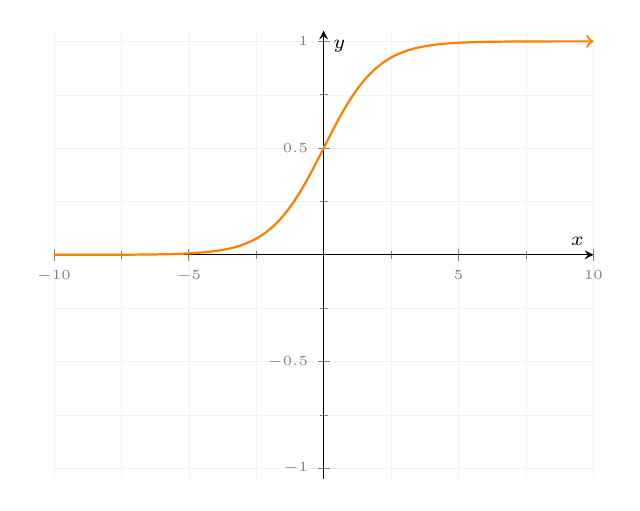
\begin{tikzpicture}
% axis settings {{{

\begin{axis}[
%	title          = graph_name,
	axis x line    = middle, % x-axis position
	axis y line    = middle, % y-axis position
	minor tick num = 1,      % num axis ticks
	grid           = both,
	grid style     =
	{
		line width=.1pt,
		draw=gray!10
	},
	xmax = 10,
	xmin = -10,
	ymax = 1.05, % 0.05 is to show the ->
	ymin = -1.05,
	tick label style = {
		font = \tiny,
		color = gray
	},
%	extra x ticks={3,1},
%	extra x tick labels={$\leftarrow$,$\rightarrow$},
%	extra y ticks={3,1},
%	extra y tick labels={$\leftarrow$,$\rightarrow$},
	legend style =
	{
		draw         = none, % remove legend bounding box
		font         = \tiny,
		legend pos   = outer north east,
		cells        = {anchor = west},
		fill         = gray,
		fill opacity = 0.4,
		text opacity = 1
	},
	xlabel       = {$\scriptstyle x$},
	ylabel       = {$\scriptstyle y$},
	xlabel style =
	{
		at     = {(ticklabel* cs:1)},
%		anchor = north west
	},
	ylabel style=
	{
		at     = {(ticklabel* cs:1)},
%		anchor = south west
	}
]
% }}}

\coordinate (O) at (0,0);

\addplot [
	domain=-10:10,
	no marks,
	samples=100,
	thick,
	orange,
	->
]
{1/(1+exp(-x)};
%\addlegendentry{$\frac{1}{1+e^{-x}}$};

\end{axis}
\end{tikzpicture}

% }}}

\[
\begin{array}{ l@{} l@{} l@{} }
	h_\theta(x)
	& = g(\theta_0 + \theta_1 x) 
	& =
	\frac{1}
	{
		1+e^
		{
			-
			\left(
				\theta_0 + \theta_1 x
			\right)
		}
	}
	\\
	h_\theta(X)
	& = g(\Theta^T X)
	& =
	\frac{1}
	{
		1+e^
		{
			-
			\left(
				\Theta^T X
			\right)
		}
	}
	\\
\end{array}
\]

\[
	\begin{array}{ l@{} l@{} }

	h_\theta(x) & = P(y=1|x;\theta)\\

	\end{array}
\]

\[
	\begin{array}{ l@{} l@{} }

	P(y=1|x;\theta) + P(y=0|x;\theta) & = 1 \\

	\end{array}
\]

\pagebreak
\subsectionend
% }}} END SUB-SECTION : hypothesis_equation
% 	SUB-SECTION : cost_function {{{
\subsection{Cost Function}
\label{ssec:cost_function}
\parindent=0em

Training set :

\[
	\begin{array}{ l@{} l@{} }
	\left\{
		\left( x^{(1)},y^{(1)} \right),
		\left( x^{(2)},y^{(2)} \right),
		\left( x^{(3)},y^{(3)} \right),
		\ldots
		\left( x^{(m)},y^{(m)} \right)
	\right\}
	\end{array}
\]

where we have m samples / examples for each data point x :

\[
	\begin{array}{ l@{} l@{} }
	\begin{bmatrix}
		x_0 \\
		x_1 \\
		\vdots \\
		x_n \\
		\end{bmatrix}
		_{1 \times(n+1)}
	\in \mathbb{R}^{n+1}
	\; , \;
	x_0 = {1}
	\; , \;
	y \in {0,1}
	\end{array}
\]



~\footnote{ Good explainer video : 
\href{ https://www.youtube.com/watch?v=XepXtl9YKwc }{https://www.youtube.com/watch?v=XepXtl9YKwc }
}



Which means that we have a new cost function $J(\theta)$:


\[
	\begin{array}{ l@{} l@{} }
	J(\theta)
	& =
	\dfrac{1}{m}
	\sum_{i=1}^m
	\left\{
		\mathrm{Cost}(h_\theta(x^{(i)}),y^{(i)})
	\right\}
	\\
	\mathrm{Cost}(h_\theta(x),y)
	& =
	\left\{
		\begin{array}{ l@{} l@{} } 
			-\log(h_\theta(x))
			\;
			& \text{if y = 1} 
			\\ 
			-\log(1-h_\theta(x))
			\;
			& \text{if y = 0} 
		\end{array}
	\right.  
	\end{array}
\]

\[
	\begin{array}{ l@{} l@{} }
		\mathrm{Cost}(h_\theta(x),y)
		&
		\left\{
		\begin{array}{ l@{} l@{} l@{} }
			& = 0
			& \text{ if } h_\theta(x) = y
			\\
			& \rightarrow \infty
			&\text{ if } y = 0
			\; \mathrm{and} \;
			h_\theta(x) \rightarrow 1
			\\
			& \rightarrow \infty
			& \text{ if } y = 1
			\; \mathrm{and} \;
			h_\theta(x) \rightarrow 0
			\\
		\end{array}
	\right.
	\end{array}
\]


	Case y = 1

	
% ln(x)  {{{

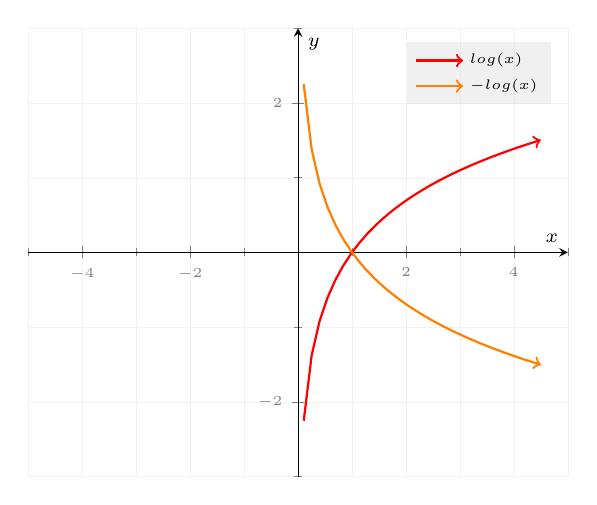
\begin{tikzpicture}
% axis settings {{{

\begin{axis}[
%	title          = graph_name,
	axis x line    = middle, % x-axis position
	axis y line    = middle, % y-axis position
	minor tick num = 1,      % num axis ticks
	grid           = both,
	grid style     =
	{
		line width = .1pt,
		draw       = gray!10
	},
	xmax      = 5,
	xmin      = -5,
	ymax      = 3,
	ymin      = -3,
	tick label style = {
		font  = \tiny,
		color = gray
	},
%	extra x ticks={3,1},
%	extra x tick labels={$\leftarrow$,$\rightarrow$},
%	extra y ticks={3,1},
%	extra y tick labels={$\leftarrow$,$\rightarrow$},
	legend style =
	{
		draw         = none, % remove legend bounding box
		font         = \tiny,
		legend pos   = north east,
		cells        = {anchor = west},
		fill         = gray!30,
		fill opacity = 0.4,
		text opacity = 1
	},
	xlabel       = {$\scriptstyle x$},
	ylabel       = {$\scriptstyle y$},
	xlabel style =
	{
		at     = {(ticklabel* cs:1)},
%		anchor = north west
	},
	ylabel style=
	{
		at     = {(ticklabel* cs:1)},
%		anchor = south west
	}
]
% }}}
\coordinate (O) at (0,0);

\addplot [
	domain=-10:4.5,
	samples=100,
	thick,
	red,
	->
]
{ln(x)};
\addlegendentry{$log(x)$};

\addplot [
	domain=-10:4.5,
	samples=100,
	thick,
	orange,
	->
]
{-ln(x)};
\addlegendentry{$-log(x)$};
\end{axis}
\end{tikzpicture}

% }}}
% ln(1-x)  {{{
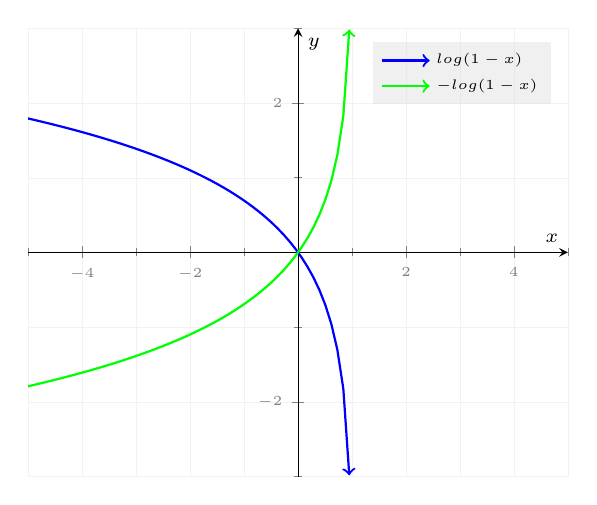
\begin{tikzpicture}
% axis settings {{{

\begin{axis}[
%	title          = graph_name,
	axis x line    = middle, % x-axis position
	axis y line    = middle, % y-axis position
	minor tick num = 1,      % num axis ticks
	grid           = both,
	grid style     =
	{
		line width = .1pt,
		draw       = gray!10
	},
	xmax      = 5,
	xmin      = -5,
	ymax      = 3,
	ymin      = -3,
	tick label style = {
		font  = \tiny,
		color = gray
	},
%	extra x ticks={3,1},
%	extra x tick labels={$\leftarrow$,$\rightarrow$},
%	extra y ticks={3,1},
%	extra y tick labels={$\leftarrow$,$\rightarrow$},
	legend style =
	{
		draw         = none, % remove legend bounding box
		font         = \tiny,
		legend pos   = north east,
		cells        = {anchor = west},
		fill         = gray!30,
		fill opacity = 0.4,
		text opacity = 1
	},
	xlabel       = {$\scriptstyle x$},
	ylabel       = {$\scriptstyle y$},
	xlabel style =
	{
		at     = {(ticklabel* cs:1)},
%		anchor = north west
	},
	ylabel style=
	{
		at     = {(ticklabel* cs:1)},
%		anchor = south west
	}
]
% }}}
\coordinate (O) at (0,0);

\addplot [
	domain=-10:0.95,
	samples=100,
	thick,
	blue,
	->
]
{ln(1-x)};
\addlegendentry{$log(1-x)$};

\addplot [
	domain=-10:0.95,
	samples=100,
	thick,
	green,
	->
]
{-ln(1-x)};
\addlegendentry{$-log(1-x)$};
\end{axis}
\end{tikzpicture}

% }}}
% ln(1-x)  {{{

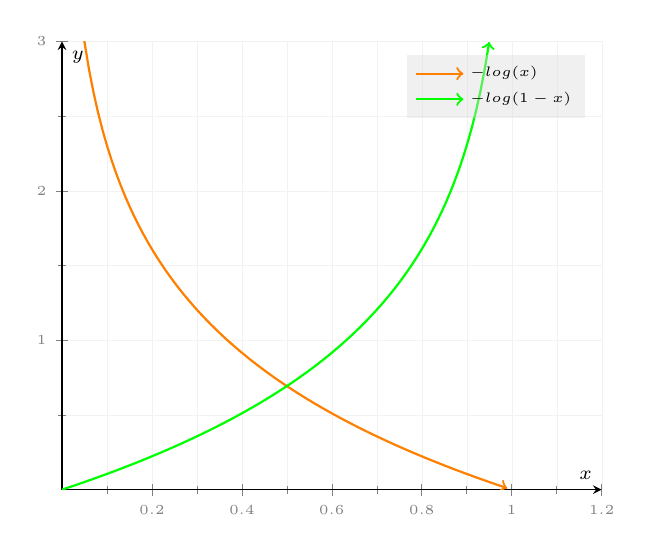
\begin{tikzpicture}
% axis settings {{{

\begin{axis}[
%	title          = graph_name,
	axis x line    = middle, % x-axis position
	axis y line    = middle, % y-axis position
	minor tick num = 1,      % num axis ticks
	grid           = both,
	grid style     =
	{
		line width = .1pt,
		draw       = gray!10
	},
	xmax      = 1.2,
	xmin      = 0,
	ymax      = 3,
	ymin      = 0,
	tick label style = {
		font  = \tiny,
		color = gray
	},
%	extra x ticks={3,1},
%	extra x tick labels={$\leftarrow$,$\rightarrow$},
%	extra y ticks={3,1},
%	extra y tick labels={$\leftarrow$,$\rightarrow$},
	legend style =
	{
		draw         = none, % remove legend bounding box
		font         = \tiny,
		legend pos   = north east,
		cells        = {anchor = west},
		fill         = gray!30,
		fill opacity = 0.4,
		text opacity = 1
	},
	xlabel       = {$\scriptstyle x$},
	ylabel       = {$\scriptstyle y$},
	xlabel style =
	{
		at     = {(ticklabel* cs:1)},
%		anchor = north west
	},
	ylabel style=
	{
		at     = {(ticklabel* cs:1)},
%		anchor = south west
	}
]
% }}}
\coordinate (O) at (0,0);

\addplot [
	domain=0:0.99,
	samples=100,
	thick,
	orange,
	->
]
{-ln(x)};
\addlegendentry{$-log(x)$};

\addplot [
	domain=0:0.95,
	samples=100,
	thick,
	green,
	->
]
{-ln(1-x)};
\addlegendentry{$-log(1-x)$};

\end{axis}
\end{tikzpicture}

% }}}

	Taking only the negative log from the graph and then using the interval
	only between $ 0 \leq x \leq 1$ , we get the following graph :

	Case y = 0
%	<img src="images/log_neg_interval.svg">
%	<img src="images/log_inv_neg_interval.svg">

\[
	\begin{array}{ l@{} l@{} l@{} } 
		\mathrm{Cost}(h_\theta(x),y)
		& = 0
		& \text{ if } h_\theta(x) = y 
		\\ 
		\mathrm{Cost}(h_\theta(x),y)
		& \rightarrow \infty
		&\text{ if } y = 0
		\; \mathrm{and} \;
		h_\theta(x) \rightarrow 1 
		\\ 
		\mathrm{Cost}(h_\theta(x),y)
		& \rightarrow \infty 
		& \text{ if } y = 1
		\; \mathrm{and} \;
		h_\theta(x) \rightarrow 0 
		\\ 
	\end{array}
\]

	\[
	\begin{array}{ l@{} l@{} } 
	J(\theta)
	& =
	\dfrac{1}{m}
	\sum_{i=1}^m
	\left\{
		\mathrm{Cost}(h_\theta(x^{(i)}),y^{(i)})
	\right\} 
	\\ 
	\mathrm{Cost}(h_\theta(x),y)
	& =
	\left\{ 
		\begin{array}{ l@{} l@{} } 
			-\log(h_\theta(x))
			\;
			& \text{if y = 1} 
			\\ 
			-\log(1-h_\theta(x))
			\;
			& \text{if y = 0} 
		\end{array}
	\right.  
	\\ 
	& = 
	-y\log(h_\theta(x))
	+
	(1-y)\log(1-h_\theta(x)) 
	\end{array}
\]


\[
	\begin{array}{ l@{} l@{} } 
	J(\theta)
	& =
	{ \displaystyle 
		\dfrac{1}{m}
		\sum_{i=1}^m
		\left\{
			\mathrm{Cost}(h_\theta(x^{(i)}),y^{(i)})
		\right\}
	}
	\\ 
	& =
	\dfrac{1}{m} 
	{ \displaystyle 
		\left(
			\sum_{i=1}^m
			\left\{
				-y^{(i)}\log(h_\theta(x^{(i)}))
				+
				(1-y^{(i)})\log(1-h_\theta(x^{(i)}))
			\right\}
		\right)
	} 
	\end{array}
\]

\[
	\begin{array}{ l@{} l@{} } 
		J(\theta)
		& =
		-
		\frac{1}{m}
		\cdot
		\sum_{i=1}^{m}
		\left\{
			y^{i}
			log(\widehat{y^{i}})
			+
			(1 - y^{i})
			log(1-\widehat{y^{i}})
		\right\}
	\end{array}
\]

\pagebreak
\subsectionend
% }}} END SUB-SECTION : cost_function
% 	SUB-SECTION : gradient_descent {{{
\subsection{Gradient Descent}
\label{ssec:gradient_descent}
\parindent=0em

\[
	\begin{array}{ l@{} l@{} }
		\nabla J(\Theta)
		& =
		\left\langle
		  {\displaystyle \frac{\partial}{\partial \theta_0} J(\Theta)}
		, {\displaystyle \frac{\partial}{\partial \theta_1} J(\Theta)}
		, {\displaystyle \frac{\partial}{\partial \theta_2} J(\Theta)}
		\ldots
		, {\displaystyle \frac{\partial}{\partial \theta_m} J(\Theta)}
		\right\rangle
		\\
	\end{array}
\]


\[
	\begin{array}{ l@{} l@{} }
\sigma(x)             & = \frac{1}{1+e^{-x}} \\
\frac{d}{dx}\sigma(x) & = \frac{d}{dx} \left(  \frac{1}{1+e^{-x} } \right) \\
                      & = \frac{0 \cdot(1+e^{-x}) - (-e^{-x}) \cdot 1}{ ( 1+e^{-x} ) ^2} \text{$\hspace{46 mm}$Quotient rule}\\
                      & = \frac{e^{-x}}{ ( 1+e^{-x} ) ^2}  \\
                      & = \frac{(1+e^{-x}) -1 }{ ( 1+e^{-x} ) ^2} \\
                      & = \frac{ (1+e^{-x})}{ ( 1+e^{-x} ) ^2}  - \left( \frac{1}{1+e^{-x}} \right)^2\\
                      & = \frac{1}{1+e^{-x}}  - \left( \frac{1}{1+e^{-x}} \right)^2\\
                      & = \sigma (x) - \sigma(x)^2\\
\sigma^{'} (x)        & = \sigma(x)(1-\sigma(x))
	\end{array}
\]


We also have the following :
\[
	\begin{array}{ l@{} l@{} } 
		h_\theta(\Theta^T x)
		= \sigma(\Theta^Tx)
		& = \frac{1}{1+e^{-\Theta^T x}} \\ 
	\end{array}
\]

\[
\begin{array}{ l@{} l@{} l@{} l@{} } 
		P(y^{(i)} = 1 | x^{(i)} ; \theta)
		& = h_\theta(x)
		& = \sigma(x)
		& = \frac{1}{1+e^{-x}}
		\\ 
		P(y^{(i)} = 0 | x^{(i)} ; \theta)
		& = 1 - h_\theta(x)
		& = 1 - \sigma(x)
		& = 1 - \frac{1}{1+e^{-x}}
		\\ 
	\end{array}
\]

This gives us the overall likelihood of any outcome y given x and theta as :

\[
\begin{array}{ l@{} l@{} l@{} } 
		L(\theta) 
		& = P(y^{(i)}| x^{(i)} ; \theta)
		& = h(x^{(i)})^{y^{(i)}} \cdot ( 1 - h(x^{(i)}))^{1 - y^{(i)}} 
	\end{array}
\]

overall i's

\[
	\begin{array}{ l@{} l@{} }
	L(\theta) & =
	{ \displaystyle \prod_{i=1}^{m} }
	\left\{
		h
		\left(x^{(i)}\right)
		^{
			\left(
				y^{(i)}
			\right)
		}
		\cdot
		\left(
			1 - h(x^{(i)})
		\right)
		^{
			\left(
				1 - y^{(i)}
			\right)
		}
	\right\}
	\\
	\log(L(\theta)) & = \mathscr{L}(\theta) \\ 
	\mathscr{L}(\theta)
	& =
	\log \left( 
	{ \displaystyle \prod_{i=1}^{m} }
	\left\{
		h
		\left(x^{(i)}\right)
		^{
			\left(
				y^{(i)}
			\right)
		} 
		\cdot 
		\left(
			1 - h(x^{(i)})
		\right)
		^{
			\left(
				1 - y^{(i)}
			\right)
		} 
	\right\} 
	\right) 
	\\ 
	& = 
	{ \displaystyle \sum_{i=1}^{m} } \left\{ 
		\log \left( 
			h
			\left(x^{(i)}\right)
			^{
				\left(
					y^{(i)}
				\right)
			} 
			\cdot 
			\left(
				1 - h(x^{(i)})
			\right)
			^{
				\left(
					1 - y^{(i)}
				\right)
			} 
		\right) 
	\right\} 
	\\ 
	& = 
	{ \displaystyle \sum_{i=1}^{m} } \left\{ 
		\log \left( 
			h
			\left(x^{(i)}\right)
			^{
				\left(
					y^{(i)}
				\right)
			} 
		\right) 
		+ 
		\log \left( 
			\left(
				1 - h(x^{(i)})
			\right)
			^{
				\left(
					1 - y^{(i)}
				\right)
			} 
		\right) 
	\right\} 
	\\ 
	& = 
	{ \displaystyle \sum_{i=1}^{m} } \left\{ 
		\left(
			y^{(i)}
		\right) 
		\cdot 
		\log \left( 
		h \left(
			x^{(i)}
		\right) 
		\right) 
		+ 
		\left(
			1 - y^{(i)}
		\right) 
		\cdot 
		\log \left( 
		\left(
			1 -
			h \left(
				x^{(i)}
			\right) 
		\right) 
		\right) 
	\right\} 
	\end{array}
\]

We want to maximize the likelihood so we take the derivative :


\[
	\begin{array}{ l@{} l@{} r@{} } 
	{ \displaystyle \frac{\partial}{\partial \theta}}
	\mathscr{L}(\theta) 
	& = 
	{ \displaystyle \frac{\partial}{\partial \theta}}
	\left(
		{ \displaystyle \sum_{i=1}^{m} } \left\{ 
			\left(
				y^{(i)}
			\right) 
			\cdot 
			\log \left( 
			h \left(
				x^{(i)}
			\right) 
			\right) 
			+ 
			\left(
				1 - y^{(i)}
			\right) 
			\cdot 
			\log \left( 
			\left(
				1 -
				h \left(
					x^{(i)}
				\right) 
			\right) 
			\right) 
		\right\}
	\right) 
	\\ 
	& = 
	{ \displaystyle \frac{\partial}{\partial \theta}}
	\left(
		{ \displaystyle \sum_{i=1}^{m} } \left\{ 
			\left(
				y^{(i)}
			\right) 
			\cdot 
			\log \left( 
			\sigma \left(
				x^{(i)}
			\right) 
			\right) 
			+ 
			\left(
				1 - y^{(i)}
			\right) 
			\cdot 
			\log \left( 
			\left(
				1 -
				\sigma \left(
					x^{(i)}
				\right) 
			\right) 
			\right) 
		\right\}
	\right) 
	\\ 
	& = 
	{ \displaystyle \sum_{i=1}^{m} } \left\{ 
		\left(
			y^{(i)}
		\right) 
		\cdot 
		{ \displaystyle \frac{\partial}{\partial \theta}} \left( 
			\log \left( 
			\sigma \left(
				x^{(i)}
			\right) 
			\right) 
		\right) 
		+ 
		\left(
			1 - y^{(i)}
		\right) 
		\cdot 
		{ \displaystyle \frac{\partial}{\partial \theta}} \left( 
			\log \left( 
			\left(
				1 -
				\sigma \left(
					x^{(i)}
				\right) 
			\right) 
		\right) 
	\right\} 
	\right) 
	\\ 
	& = 
	{ \displaystyle \sum_{i=1}^{m} } \left\{ 
		\left(
			y^{(i)}
		\right) 
		\cdot 
		\left( 
			{ \displaystyle
			\frac
				{
					1
				}
				{
					\sigma \left( x^{(i)} \right)
				}
			} 
			\cdot 
			\sigma \prime \left( x^{(i)} \right) 
		\right) 
		+ 
		\left( 1 - y^{(i)} \right) 
		\cdot 
		\left( 
			{ \displaystyle
			\frac
				{
					1
				}
				{
					1 - \sigma \left( x^{(i)} \right)
				}
			} 
			\cdot 
			- \sigma \prime \left( x^{(i)} \right) 
		\right) 
	\right\} 
	& \text{Chain Rule} 
	\\ 
	& = 
	\end{array}
\]

Gradient Descent

\[
	\begin{array}{ l@{} l@{} } 
		\frac{\partial}{\partial \theta_0} J(\Theta)
		& =
		\left(
			\frac{1}{m}
			\cdot
			\sum_{i=1}^m \left\{
					\left(
						h_\theta(x^{(i)}) - y^{(i)}
					\right)^{2}
					\cdot
					x_{0}^{(i)}
			\right\}
		\right) 
		\\ 
		\frac{\partial}{\partial \theta_j} J(\Theta)
		& =
		\left(
			\frac{1}{m} \cdot
			\sum_{i=1}^m \left\{
				\left(
					h_\theta(x^{(i)}) - y^{(i)}
				\right)^{2}
				\cdot
				x_{j}^{(i)}
			\right\}
		\right) 
		+ 
		\frac{\lambda}{m}\cdot \theta_j 
		\\ 
	\end{array}
\]

The second sum, 
\( \frac{\lambda}{2m}
   \sum_{j = 1}^{n} {\theta_{j}^{2}} \)
means to explicitly exclude the bias term, $\theta_0$. i.e. the $\theta$
vector is indexed from 0 to n (holding n+1 values, $\theta_0$ through
$\theta_n$), and this sum explicitly skips $\theta_0$, by
running from 1 to n, skipping 0. Thus, when computing the equation, we should
continuously update the two following equations:

	\[
	\begin{array}{ l@{} l@{} l@{} l@{} } 
		\theta_0
		& := &
		\theta_0
		- \alpha
		\cdot
		\left(
		\frac{1}{m}
		\cdot 
			\sum_{i=1}^m
			\left\{
				\left(
					h_\theta(x^{(i)}) - y^{(i)}
				\right)^{2}
				\cdot
				x_{0}^{(i)}
			\right\}
		\right) 
		\hspace{0.5cm} & \text{for} \; j = 0 
		\\ 
		\theta_j
		& := &
		\theta_j
		- \alpha
		\cdot
		\left(
		\frac{1}{m}
		\cdot 
			\sum_{i=1}^m
			\left\{
				\left(
					h_\theta(x^{(i)}) - y^{(i)}
				\right)^{2}
				\cdot
				x_{j}^{(i)}
				+
				\left(
					\frac{\lambda}{m}\cdot \theta_j
				\right)
			\right\}
		\right) 
		\hspace{0.5cm} & \text{for} \; j = 1,2, \ldots , n 
		\\ 
		& :=
		& \theta_j
		\cdot
		(1 - \alpha \cdot \frac{\lambda}{m})
		-
		\alpha
		\cdot
		\left(
		\frac{1}{m}
		\cdot 
			\sum_{i=1}^m
			\left\{
				\left(
					h_\theta(x^{(i)}) - y^{(i)}
				\right)^{2}
				\cdot
				x_{j}^{(i)} 
			\right\}
		\right) 
		\\ 
		\end{array}
	\]

Using gradient descent the gradient vector is :

\[
	\begin{array}{ l@{} l@{} } 
		\nabla J
		& = 
		\begin{bmatrix} 
			\frac{\partial J(\theta_1)}{\partial \theta_1}  \\ 
			\frac{\partial J(\theta_2)}{\partial \theta_2}  \\ 
			\vdots \\ 
			\frac{\partial J(\theta_k)}{\partial \theta_k}  \\ 
		\end{bmatrix} 
	\end{array}
\]

\[
	\begin{array}{ l@{} l@{} } 
		\frac{\partial}{\partial \theta_0} J(\theta_1)
		& =
		-
		\frac{1}{m}
		\cdot 
		\sum_{i=1}^m
		\left\{
			\left(
				y^{i} - \widehat{y^{i}}
			\right)
			\cdot
			x_{1}^{i}
		\right\} 
	\end{array}
\]


\pagebreak
\subsectionend
% }}} END SUB-SECTION : gradient_descent
% 	SUB-SECTION : update_rule {{{
\subsection{Update Rule}
\label{ssec:update_rule}
\parindent=0em

\[
	\begin{array}{ l@{} l@{} } 
	\theta_{new} = \theta_{prev} - \eta \nabla J 
	\end{array}
\]

\subsectionend
% }}} END SUB-SECTION : update_rule

% 	SUB-SECTION : extra {{{
\subsection{Extra}
\label{ssec:extra}
\parindent=0em

% 		SUB-SUB-SECTION : multiclass_classification {{{
\subsubsection{Multiclass Classification}
\label{sssec:multiclass_classification}
\parindent=0em

		\[
			\begin{array}{ l@{} l@{} }
				h_\theta^{(i)}(x) = P(y=i|x;\theta) \; , \; 1 \leq i \leq k , k
				\in \mathbb{N}
			\end{array}
		\]

		
		\[
			\begin{array}{ l@{} l@{} }
				\max\limits_i h_\theta^{(i)}(x) &
			\end{array}
		\]

\pagebreak
\subsubsectionend
% }}} END SUB-SUB-SECTION : multiclass_classification
% 		SUB-SUB-SECTION : overfitting {{{
\subsubsection{Overfitting}
\label{sssec:overfitting}
\parindent=0em

	\[
		\begin{array}{ l@{} l@{} }


			J(\theta)
			= \frac{1}{2m}
			\sum_{i=1}^m
			\left\{
				\left(
					h_\theta(x^{(i)}) - y^{(i)}
				\right)^{2}
			\right\}

			\approx 0


		\end{array}
	\]

\pagebreak
\subsubsectionend
% }}} END SUB-SUB-SECTION : overfitting
% 		SUB-SUB-SECTION : regularization {{{
\subsubsection{Regularization}
\label{sssec:regularization}
\parindent=0em


\[
	\begin{array}{ l@{} l@{} } 
		\frac{1}{2} \cdot
		\frac{1}{m} \cdot 
		\lambda \cdot
		\sum_{j = 1}^{n}
		\left\{
			{\theta_{j}^{2}}
		\right\} 
	\end{array}
\]

$\lambda$ is called the regularization parameter. Its job is to control the
tradeoff between two different goals. The first goal is to actually fit the
training data well. This is done by our original cost function $J(\theta)$. The
second goal is to keep the parameters small. 

\[
	\begin{array}{ l@{} l@{} } 
		J(\theta)
		=
		\left( 
		\frac{1}{2}
		\cdot
		\frac{1}{m}
		\cdot 
			\left(
				\sum_{i=1}^m
				\left\{
					\left(
						h_\theta(x^{(i)}) - y^{(i)}
					\right)^{2}
				\right\}
			\right) 
			+
			\left( 
				\frac{1}{2} \cdot
				\frac{1}{m} \cdot 
				\lambda \cdot
				\sum_{j = 1}^{n}
				\left\{
					{\theta_{j}^{2}}
				\right\}
			\right)
		\right) 
	\end{array} 
\]

\[
	\begin{array}{ l@{} l@{} } 
		\min\limits_\theta
		J(\theta)
		=
		\frac{1}{2}
		\cdot
		\frac{1}{m}
		\cdot
		\left(
			\left(
				\sum_{i=1}^m
				\left\{
					\left(
						h_\theta(x^{(i)}) - y^{(i)}
					\right)^{2}
				\right\}
			\right) 
			+
			\left( 
				\frac{1}{2} \cdot
				\frac{1}{m} \cdot
				\lambda \cdot
				\sum_{j = 1}^{n}
				\left\{
					{\theta_{j}^{2}}
				\right\}
			\right)
		\right) 
	\end{array} 
\]


\subsubsectionend
% }}} END SUB-SUB-SECTION : regularization

\pagebreak
\subsectionend
% }}} END SUB-SECTION : extra

%\sectionend
% }}} END SECTION : logistic_regression
   \clearpage


\onecolumn
% SECTION : linear_regression {{{
\section{Linear Regression}
\label{sec:linear_regression}
\parindent=0em

% 	SUB-SECTION : univariate_linear_regression {{{
\subsection{Univariate Linear Regression}
\label{ssec:univariate_linear_regression}

% 		SUB-SUB-SECTION : motivation {{{
\subsubsection{Motivation}
\label{sssec:motivation}


\lettrine[lines=3, findent=3pt, nindent=0pt]{T}{he} problem that we are trying
to solve with most machine learning algorithms is that we are basically trying
to predict some new information based on some old information that we already
know. So what we want is some mathematical model that given some previous
information can tell us with a high degree of probability where any new
information might lie. There are many ways to do this , but here we are going to
discuss only the most basic form of a model which is a line. Or more
specifically if you remember from high school classes this would be the line of
best fit. Basically if we have a 2-D scatter plot , we just find the line of
best fit for this scatter plot and we're done.\\

One of the cliché basic machine learning problems is trying to predict housing
prices. If the example isn't broken , I'm not going to fix it for sake of novelty
, so I'm just going to stick to the same example. Let us say that we have a set
of housing prices ($y$) , and a set of house sizes ($x$). What we want is a
model that based on any new housing price $x_{new}$ would tell us what the price
should be based on all of our historical prices. All we do is make a scatter
plot of out existing data points and find the line of best fit. Pretty
simple.\\

This is basically what univariate linear regression is and hopefully we now have
a good understanding of why we are doing what we are doing. So now lets get to
the how.\\

\subsubsectionend
% }}} END SUB-SUB-SECTION : motivation
% 		SUB-SUB-SECTION : equation {{{
\subsubsection{Hypothesis Equation}
\label{sssec:equation}

The first thing to do is recall the equation of a line from our elementary
school days. It was of the form \( y=mx+b \) , but we want to be fancy machine
learning programmers now , so we want to use things like functions and Greek
symbols.  ~\footnote{This is only meant facetiously. I thought I should put in
	this note in case someone reads this and gets put off or something about
	the sarcasm.  } So our y-intercept \( b \) becomes \( \theta_{0} \) , our
slope \( m \) becomes \( \theta_{1} \) and \( y \) becomes \( h_{\theta}(x) \).
The \( x \) stays as \( x \).\\

From now on, I will never refer to the highschool version of the equation of a
line again, since it has a \( y \) in it, and this is likely to cause
confusion when talking about our \( y \) values from the \( (x,y) \) data
points. So to reiterate the \( y \) from this point forward has nothing to do
with the equation of a line, that was only used to help you understand the new
notation by comparing it to something familiar.\\

The function is \( h(x) \) is called a \textbf{\textit{Hypothesis function}}.
Given a input value \( x \) , the hypothesis function denotes the corresponding
\textbf{\textit{predicted value}} \( \hat{y} = h(x) \). The \( \hat{y} \) is
often more used in statistics and math while \( h(x) \) is more used in machine
learning , people's usage of one or the other tends to imply basically where
they first learned this linear regression concept , either in a statisics class
or in a computer science class. These \( \hat{y} = h(x) \) values are also
sometimes referred to as \textbf{\textit{target variables}} or
\textbf{\textit{output variables}}.  \\

To maintain complete clarity and refer back to our housing price example
, \( y \) are the housing prices we already know. The \( \hat{y} \) is the
house price that we guess based on our linear regression line and a new house
square footage \( x \).

This gives us our equation for the hypothesis function :

\[ h_{\theta}(x) = \theta_{0} + \theta_{1} \cdot x \tag{1} \]

or more formally :

\[
	\begin{aligned}
		h : x^{(i)} \rightarrow y^{(i)}
		& , &
		x^{(i)} \in X=\{x_1 , \ldots , x_m \}
		\\
	\end{aligned}
\]

such that \( h_{\theta}(x) \)  is a good predictor for the corresponding
value of y for a training example of \( (x,y) \).

Here we only have one variable \( x \) which is namely the size of our houses
from the earlier example. This variable \( x \) is commonly known as our
\textbf{\textit{input variable}} or a \textbf{\textit{feature}}. This is a model
based on only one feature or variable , which is why this technique is called
\textbf{uni}variate linear regression.  Later we can use not only the house size
, but also the number of bedrooms that house has , the number of bathrooms ,
whether or not the house has a yard , and so on as multiple variables to use in
our model. But for now lets just stick with the one that we have. \\

We usually split our data into two sets the \textbf {training set} , and the
\textbf {test set}. The training set is what we use to build our line of best
fit , and the test set as the name implies is used to test how well our model
is working. Each data point is basically a \( (x,y) \) pair of values. 

A summary of all the notation for this section is given below :

% TABULAR TABLE : univariate_regression_notation {{{

%\tabulartable
%{ 0.5\columnwidth }
%{ lll }
%{
%Input Variable                   & : & \( x \) \\
%Output Variable                  & : & \( y \) \\
%Training Example                 & : & \( (x,y) \) \\
%\( i^{th} \) training example    & : & \( ( x^{(i)} , y^{(i)} ) \) \\
%Training Set                     & : & \( i = 1 , \ldots , m \) \\
%Number of training examples      & : & \( m \) \\
%Hypothesis Function / Prediction & : & \( h_{\theta}(x) \) / \( \hat{y} \) \\
%Slope                            & : & \( \theta_1 \) \\
%Intercept                        & : & \( \theta_0 \) \\
%Learning Rate                    & : & \( \alpha \) \\

%}


% }}} End TABULAR TABLE :  Univariate Regression Notation


\subsubsectionend
% }}} END SUB-SUB-SECTION : equation
% 		SUB-SUB-SECTION : cost_function {{{
\subsubsection{Cost Function}
\label{sssec:cost_function}

OK , now we know the `form' of the function which is \( h_{\theta}(x) =
	\theta_{0} + \theta_{1}x  \). We now have to learn this function.  But what
does `learning' a function mean ? To do understand this look at the graph below
, each line here denotes a possible h value : \\

% tkiz two column {{{

\begin{figure}[h!]

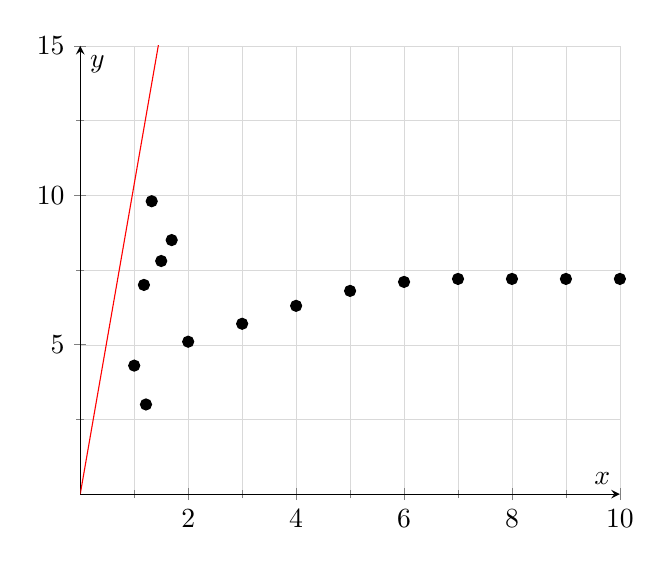
\begin{tikzpicture}
\pgfplotsset{
	every axis legend/.append style={
	at={(0.5,1.03)},
	anchor=south
},
}
\begin{axis}[
%	title          = log(x) / - log(x),
	axis x line    = middle, % x-axis post
	axis y line    = middle, % y-axis post
	minor tick num = 1,      % num axis ticks
    grid           = both,
    grid style     =
	{
		line width=.1pt,
		draw=gray!30
	},
    xmax=10,
    xmin=0,
    ymin=0,
    ymax=15,
	% more plot options in manual for pgfplots
	legend style =
	{
		draw = none % remove legend bounding box
	},
	xlabel       = {$x$},
	ylabel       = {$y$},
	scatter/classes={
		a = { mark=o , draw=black}
	}
]

\addplot [color=red, domain=0:15, mark=none] {0.0051026+10.372231*\x};

\addplot[
	scatter,
	only marks,
    scatter src=explicit symbolic
]
table[meta=label]
{
		x y label
		1 4.3 a
		2 5.1 a
		3 5.7 a
		4 6.3 a
		5 6.8 a
		6 7.1 a
		7 7.2 a
		8 7.2 a
		9 7.2 a
		10 7.2 a
		11 7.5 a

		1.218 3 a
		1.18 7 a
		1.694 8.5 a
		1.324 9.8 a
		1.5 7.8 a

		12 7.8 a
		12 7.8 a
		12 7.8 a
		12 7.8 a
		12 7.8 a
		12 7.8 a
		12 7.8 a
		12 7.8 a
		12 7.8 a
		12 7.8 a
		12 7.8 a
		12 7.8 a
};
\end{axis}
\end{tikzpicture}


\caption{}
\label{fig:placeholder}
\end{figure}
% }}}

Learning here means figuring out which one of the lines drawn ( and many many
more not drawn ) should we use as our hypothesis function ? Or rather given all
the lines , which one of them is the BEST FIT line to our data points.\\

In our equation we already have a fixed value \( x \) , so we need to figure out
what is the best y-intercept \( \theta_0 \) , and slope \( \theta_1 \).
Therefore our learning task now becomes , out of all possible real values , what
are the values of \( \theta_0 \) and \( \theta_1 \) , such that the difference
between our guessed value \( h(x) \) and our known value \( y \) is as small as
we can make it , i.e. , we want the value of \( h_{\theta}(x) - y \) to be as
small as possible , and ideally 0.\\

Keep in mind , that here for every change in our theta values , the distance 
\( h_{\theta}(x) - y \) will change for all of our \( y^{(i)} \)'s in our
training set and we want a \( h(x) \) so that the distance is as small as it can
be for all of the \( y^{(i)} \) not just 0 for one and some large number for all
the others.\\

These \( \theta_{i} \) values are called \textbf{\textit{parameters}}, and what
we need to do is guess good values for these parameters. We need something that
tells us whether the values we choose are `good' or not. This something is
called an \textbf{evaluation metric}. Evaluation Metrics are used to explain
the performance of a model. They compare the difference between the real value
and the predicted value of a model. There are a lot of different equations that
we can use as our evaluation metric. Each has its own pro's and con's. Some of
the most commonly used ones are : 

\textbf{\textit{Mean Absolute Error}}
\[
\text{} \\
\textbf{MAE} =
	\frac{1}{n}
	\cdot \sum_{j=1}^{n}
	\left\{
		| y_j - \hat{y_j} |
	\right\}
	\\
\]

\textbf{\textit{Mean Squared Error}}

Mean squared error is popular because the focus of the error is geared towards
larger errors. This is due to the squared term exponentially increasing larger
errors in comparison to smaller ones.

\[
\textbf{MSE} = 
	\frac{1}{n}
	\cdot \sum_{i=1}^{n}
	\left\{
		\left(
			y_i - \hat{y_i}
		\right)^2
	\right\}
	\\
\]

\textbf{\textit{Root Mean Squared Error}}

Root Mean squared error is also very popular since it is interpretable in the
same units as the response vector. Which makes it easy to relate its
information.

\[
	\textbf{RMSE} =
	\sqrt[2]
	{
		\frac{1}{n}
		\cdot \sum_{i=1}^{n}
		\left\{
			\left(
				y_i - \hat{y_i}
			\right)^2
		\right\}
	}
	\\
\]

\textbf{\textit{Relative Absolute Error}}

The Relative Absolute Error , also known as the Residual Sum of Square , takes
the total absolute value and normalizes it by dividing by the absolute sum of
the simple predictor. \\

\[
	\textbf{RAE} =
		\frac
		{
		\sum_{j=1}^{n}
		\left\{
			|y_{j} - \hat{y_j}|
		\right\}
		}
		{
		\sum_{j=1}^{n}
		\left\{
			|y_{j} - \hat{y}|
		\right\}
	}
	\\
\]

\textbf{\textit{Relative Squared Error }}
\[
\begin{aligned} 
	\textbf{RSE} & =
	\frac
	{ 
	\sum_{j=1}^{n}
	\left\{
		\left(
			y_{j} - \hat{y_j}
		\right)^2
	\right\}
	}
	{
	\sum_{j=1}^{n}
	\left\{
		\left(
			y_{j} - \hat{y}
		\right)^2
	\right\}
	}
	\\
	R^2 & = 1 - RSE \\
\end{aligned}
\]

For the sake of this writeup I will be using the \textbf{Mean Squared Error}.
The reason is that based on previous evidence of hundreds of times doing this
with other cost functions , the square error function is a reasonable choice
that works well for most regression problems.

The equation is given again below :

\[ MSE = \frac{1}{n} \sum_{i=0}^{n} \{ ( \hat{y_{i}} - y_{i} ) ^{2} \} \]

This is the `generic' or statistics version of the equation , which means that I
have not used the machine learning variable forms in it. I wanted to show it in
this form first. Because after this point we'll probably be staring at the other
version for a long while. \\

The computer science version of the same mean squared error equation is commonly
called the \textbf{\textit{cost function}} and is represented using the
character \( J \). The function is defined as follows :

\[
\begin{aligned}
	J(\theta_{0}, \theta_{1}) & = 
	\frac{1}{2}
	\cdot \frac{1}{m}
	\cdot \sum_{i=0}^{m}
	\{
( h_{\theta}(x)^{(i)} - y^{(i)} )^{2}
\} \\
\end{aligned}
\tag{2}
\]

Keep in mind here are that the superscripts \( (i) \) are not powers they are
indexes into our training set , so dont get confused. \\

Oh , also note here that we multiply by the additional term \( \frac{1}{2} \).
It doesnt really change much about the equation it just scales the values down ,
but it helps a lot in cleaning up the gradient descent calculations that we are
just about to do. \\

Speaking of gradient descent , what in the world is that ? Keep in mind that so
far , our function \( J(\theta_{0}, \theta_{1}) \)  only represents how much
error there is in our guesses for \( \theta_0 \) and \( \theta_1 \). But our job
doesn't end here , we actually have to minimize this error value and keep making
our model better. Therefore our task now becomes to minimize the cost function
\( J \) : 

\( \min_{ \theta_0 , \theta_1 } J(\theta_0,\theta_1) \)

and the algorithm we are going to use to minimize this function is gradient
descent. \\


\subsubsectionend
% }}} END SUB-SUB-SECTION : cost_function
% 		SUB-SUB-SECTION : gradient_descent {{{
\subsubsection{Gradient Descent}
\label{sssec:gradient_descent}

\lettrine[lines=3, findent=3pt, nindent=0pt]{G}{radient} Descent is an algorithm
that solves our minimization problem. It is sometimes also called the hill
climbing algorithm, but that is just a naming convention depending on what your
source of learning is. I'm just gonna stick with gradient descent since going
downhill I feel is preferable to going uphill. This algorithms main job
is reduce the value of any given function to a minimum value based on some given
parameters.  Gradient descent works not only for linear regression but for all
sorts of minimization problems in machine learning. Minimizing the cost function
for linear regression is only one small application of gradient descent.

We are dealing with univariate linear regression right now, but the same
algorithm would work in the multivariate case , i.e. , over an arbitrary number
of parameters \( \theta_0 , \theta_1 , \ldots , \theta_n \). This is useful to
know for the future , but for right now we will only be minimizing with respect
to our two parameters \( \theta_0 \) and \( \theta_1 \) , i.e. , we are going to
be running gradient descent on our linear regression cost function \(
	J(\theta_0,\theta_1) \).

\textbf{\textit{Intuition}}

Try to imagine yourself standing on top of a grassy hill. You now want to get
back downhill. What is the easiest and fastest way to do that ?  You can just
look around 360° , and take a step in which ever direction seems to have the
biggest slope downhill.  This seems like best most intuitive way to ensure that
at every moment you are constantly heading downhill.

One caveat to mention here is that you are also extremely short sighted
so you can only see enough for one step forward , so you cannot go up for a
while for a bigger descent later.

This is basically what gradient descent algorithm does. More formally
the algorithm is defined as follows :

\[ 
\begin{aligned} 
	& \text{repeat until convergence  }
	\{ \\ 
	& \hspace{0.5cm}
	\theta_j :=
	\theta_j
	- \alpha
	\cdot \frac{\partial}{\partial \theta_j} J(\theta_0,\theta_1) 
	\hspace{0.5cm} 
	\text{(for j=0 and j=1)} 
	\\
	&
	\} \\
\end{aligned}
\]

Convergence means that after running the algorithm another time , the
value of \( theta_j \) will not change. In practice however we basically wait
until there is no \textbf {significant} change in our value for \( \theta_j \).
This is because it might not be worth waiting around for another day or a week
just to get another 0.0001\% increase in accuracy for your model. As the machine
learning engineer it would be up to you to decide how accurate you want it to be
and how long you are willing to wait for it get that accurate.\\

Also note that in the equation above := indicates assignment and not equality.\\



%We have two variables to optimize over \( \theta_0 \) and \( theta_1 \) , but
%for sake of explanation and illustration , it is easier to remain in the 2-D
%plane.  So we reduce the equation down to only using \( \theta_1 \) , the
%problem is therefore :

%\[
%\begin{aligned}
%\min_{\theta_1} J(\theta_1)
%\hspace{0.5cm}
%\theta_1 \in \mathbb{R}
%\end{aligned}
%\]

%\[
%\begin{aligned}
%\theta_1 := \theta_1 - \alpha
%\cdot \frac{\partial}{\partial \theta_1} J(\theta_1)
%\end{aligned}
%\]

Following is the caculation of the partial derivative term from the
gradient descent algorithm for linear regression.

\[
\begin{aligned}
	&\frac{\partial}{\partial \theta_j}
	J(\theta_{0}, \theta_{1}) \\
	& =
	\frac{\partial}{\partial \theta_j}
	\left(
		\frac{1}{2}
		\cdot \frac{1}{m}
		\cdot \sum_{i=0}^{m}
			\left\{
				\left(
					h_{\theta}(x)^{(i)} - y^{(i)}
				\right)^{2}
			\right\}
	\right)
	\\
	& =
	\frac{\partial}{\partial \theta_j}
	\left(
		\frac{1}{2}
		\cdot \frac{1}{m}
		\cdot \sum_{i=0}^{m}
			\left\{
				\left(
					\left(
						\theta_{0} + \theta_{1} \cdot x^{(i)}
					\right)
					- y^{(i)}
				\right)^{2}
			\right\}
	\right)
	\\
\end{aligned}
\]

This is straighforward because we only have to do the differential for two
values of $\theta_j$ , namely $\theta_0$ and $\theta_1$ : 

\[
\begin{aligned}
	& \frac{\partial}{\partial \theta_0} J(\theta_{0}, \theta_{1}) \\
	& =
	\frac{\partial}{\partial \theta_0}
	\left(
		\frac{1}{2}
		\cdot \frac{1}{m}
		\cdot \sum_{i=0}^{m}
			\left\{
				\left(
					\left(
						\theta_{0} + \theta_{1} \cdot x^{(i)}
					\right)
					- y^{(i)}
				\right)^{2}
			\right\}
	\right)
	\\
	& =
	\phantom{ \frac{\partial}{\partial \theta_0} }
	% align parenthesis 
	\left(
		\frac{1}{m}
		\cdot \sum_{i=0}^{m}
			\left\{
				\left(
					h_{\theta}(x)^{(i)} - y^{(i)}
				\right)^{2}
			\right\}
	\right)
	\\
\end{aligned}
\]

\[
\begin{aligned}
	& \frac{\partial}{\partial \theta_1} J(\theta_{0}, \theta_{1}) \\
	& =
	\frac{\partial}{\partial \theta_1}
	\left(
		\frac{1}{2}
		\cdot \frac{1}{m}
		\cdot \sum_{i=0}^{m}
			\left\{
				\left(
					\left(
						\theta_{0} + \theta_{1} \cdot x^{(i)}
					\right)
					- y^{(i)}
				\right)^{2}
			\right\}
	\right)
	\\
	& =
	\phantom{ \frac{\partial}{\partial \theta_0} }
	% align parenthesis
	\left(
	\frac{1}{m}
	\cdot \sum_{i=0}^{m}
		\left\{
			\left(
				h_{\theta}(x)^{(i)} - y^{(i)}
			\right)^{2}
		\right\}
	\right)
	\cdot (x)^{\left(i\right)}
	\\
\end{aligned}
\]

Now that we have a way of getting new and improved \( \theta_0 \) and \(
	\theta_1 \) values , we have to actually somehow put these new values into
our old equation. This means that we need an update rule.


\subsubsectionend
% }}} END SUB-SUB-SECTION : gradient_descent
% 		SUB-SUB-SECTION : update_rule {{{
\subsubsection{Update Rule}
\label{sssec:update_rule}

One thing to keep in mind when implementing gradient descent , is the correct
order of the parameter update operation. We want to update our parameters
all at the same time , because if we dont do that then we are running gradient
descent on an effectively different paramter set than the one we want to
optimize over.

Following is the \textbf{INCORRECT} way of implementing the update rule :

\[
\begin{aligned}
	temp0 &:= \theta_0 - \alpha
	\cdot \frac{\partial}{\partial \theta_0} J(\theta_0,\theta_1) \\
	\theta_0 &:= temp0 \\
	temp1 &:= \theta_1 - \alpha
	\cdot \frac{\partial}{\partial \theta_1} J(\theta_0,\theta_1) \\
	\theta_1 &:= temp1 \\
\end{aligned}
\]

Following is the \textbf{CORRECT} way to implement a simultaneous update.

\[
\begin{aligned}
	temp0 &:= \theta_0 - \alpha
	\cdot \frac{\partial}{\partial \theta_0} J(\theta_0,\theta_1) \\
	temp1 &:= \theta_1 - \alpha
	\cdot \frac{\partial}{\partial \theta_1} J(\theta_0,\theta_1) \\
	\theta_0 &:= temp0 \\
	\theta_1 &:= temp1 \\
\end{aligned}
\]

Basically do all your calculations before you do all your assignments.\\

This update rule marks the end of our basic univariate linear regression
algorithm.\\

\subsubsectionend
% }}} END SUB-SUB-SECTION : update_rule

\subsectionend
% }}} END SUB-SECTION : univariate_linear_regression

% 	SUB-SECTION : multivariate_linear_regression {{{
\subsection{Multivariate Linear Regression}
\label{ssec:multivariate_linear_regression}

% 		SUB-SUB-SECTION : motivation {{{
\subsubsection{Motivation}
\label{sssec:motivation}

The motivation at this point is to generalize our existing linear regression
algorithm. This means that we want to get out of two dimensions where we are
only using the equation of a line and two parameters \( \theta_0 \) and \(
	\theta_1 \) , and build a version of linear regression that can use an
arbitrary number of parameters \( \theta_0 , \theta_1 , \ldots , \theta_n \).
This means that we are going to have a whole bunch of equations , and a whole
bunch of derivatives we are going to have to calculate when doing gradient
descent. Since we have to solve a large number of equations simultaneously , the
best way would be to use Matrices because that is kind of their raison d'être.\\

But before we do any calculations , we need to transform our existing
equations into their new vector / matrix forms and deal with some more
notation.\\


\subsubsectionend
% }}} END SUB-SUB-SECTION : motivation
% 		SUB-SUB-SECTION : equation {{{
\subsubsection{Hypothesis Equation}
\label{sssec:equation}

 Independant / Input Variable / Feature : $ x\; $ 

 Number of features $x$ : $ n\; , \; n \in \mathbb{N} $ 

 Output Variable / Dependant Variable / Target : $ y\; $ 

 Number of training examples $y$ : $ m  \; , \; m \in \mathbb{N} $ 

  the $j^{th}$ feature : $ x_{j} $ for $ j \in \{1 , \ldots , n\} $ , where features are columns in a table

  the $i^{th}$ training set / vector : $x^{(i)}$  for $ i \in \{1 , \ldots , m\} $ $\; , \;  x^{(i)} \in \mathbb{R}^{n} $
 , where indexes are rows in a table

  value of feature $j$ in $i^{th}$ training example : $ x_{j}^{(i)} $ , 
 in an $ m \times n$ data table it is the value of the $i^{th}$ row , $j^{th}$ column 

 $i^{th}$ training example : $ ( x_{j}^{(i)} , y^{(i)} ) $ 
 Learning Rate : \( \alpha \) 
So continuing with our housing prices example from univariate linear regression.
Let us now assume that we have a dataset of housing prices , for four houses
\(x_0, x_1 , x_2 , x_3 \). We can represent these in a 1-dimensional vector as
follows :

\[
X =
\text{Housing Prices}  =
\begin{bmatrix}
	x_0 \\
	x_1 \\
	x_2 \\
	x_3 \\
\end{bmatrix}
\]

We want to do linear regression , i.e. , we want to figure out house prices in
the future given data we already have.

In addition to the prices of the house , we have two features that we know
affect the house price. Lets assume they are square footage , and number of
bedrooms. These can be represented by the \( \theta_0 \) , and \( \theta_1 \)
respectively. So far everything look similar to what we have seen before. But
this time , the only difference from what we did in univariate regression
earlier is that instead of just having one \( x \) , we have multiple \(x_0, x_1
	, x_2 , x_3 \) values represented in a vector \( X \). Which means that we
have multiple hypothesis equations :

\[
	\begin{array}{ l@{} l@{} }
		h_{\theta}(x_0) &= \theta_{0} + \theta_{1}x_0  \\
		h_{\theta}(x_1) &= \theta_{0} + \theta_{1}x_1  \\
		h_{\theta}(x_2) &= \theta_{0} + \theta_{1}x_2  \\
		h_{\theta}(x_3) &= \theta_{0} + \theta_{1}x_3  \\
	\end{array}
\]

What we want to do , is to represent all the equations above in one succinct
form. To do this we need 1 vector for each one of our features \( \theta \) ,
and 1 for all our input variables \( X \). The challenge right now is that we
have to split up \( \theta_{1}x \), into an independent \( X \) vector and \(
	\theta_1 \) vector , so that we can represent this multiplication in terms
of matrices.\\

So first step is to transform our 1-D Housing prices vector (\( X \)) to a 2-D
matrix  :

\[
\begin{array}{ l@{} l@{} l@{} l@{} l@{}} 
\begin{bmatrix}
	1 & x_0 \\
	1 & x_1 \\
	1 & x_2 \\
	1 & x_3 \\
\end{bmatrix}

\end{array}
\]

Second step , represent , our parameter values as a vector

\[
	\begin{array}{ l@{} l@{} }
		\begin{bmatrix}
			\theta_0 \\
			\theta_1 \\
		\end{bmatrix} 
	\end{array}
\]

Now we do matrix multiplication which easily and succinctly gives us our
predicted $ h_{\theta}(x) $ values for all four house prices.

\[
\begin{array}{ l@{} l@{} l@{} l@{} l@{} l@{}}
Prediction
& =
& Data
& \times
& Parameters \\
\begin{bmatrix}
	h_{\theta}(x_0) \\
	h_{\theta}(x_1) \\
	h_{\theta}(x_2) \\
	h_{\theta}(x_3) \\
\end{bmatrix}
& =
& \begin{bmatrix}
	1 & x_0 \\
	1 & x_1 \\
	1 & x_2 \\
	1 & x_3 \\
\end{bmatrix}
& \times
& \begin{bmatrix}
	\theta_0 \\
	\theta_1 \\
\end{bmatrix}
\\
& =
& \begin{bmatrix}
	( \theta_0 \cdot 1 ) + (\theta_1 \cdot x_0) \\
	( \theta_0 \cdot 1 ) + (\theta_1 \cdot x_1) \\
	( \theta_0 \cdot 1 ) + (\theta_1 \cdot x_2) \\
	( \theta_0 \cdot 1 ) + (\theta_1 \cdot x_3) \\
\end{bmatrix}
\\
\end{array}
\]

Not only is this form cleaner to look and more efficient to solve. It provides a
huge advantage in that we can optimize our parameters , and minimize the cost
function equation $ J(\theta_0 , \ldots , \theta_n) $ very efficiently without
having to go through an iterative process using gradient descent like we were
doing earlier in univariate linear regression.\\

Which means that the more input variables and features that we have , the more
this matrix multiplication method becomes useful and at a certain point in fact
necessary. Not to mention the matrix notation tends to take up less space and
look cleaner so a bunch of people prefer it. It can make you want to tear your
hair out if you haven't completely understood what is going on though. kek.
Which is the exactly why I am sitting here going line by line and typing it all
out.  Mainly for me to understand it but on the one in a billion chance that
anyone else actually reads this , then also for the sake your hairline.\\

Now that we understand how it works for a finite number of houses \( x_0 ,
\ldots , x_3 \) , and parameters \( \theta_0 \) , \( \theta_1 \) , our job
is to now transform this further into an equation for an arbitrary number of
input vectors (houses) \( x_0 , x_1 , \ldots , x_n \) , and an arbitrary number
of parameters \( \theta_0 , \theta_1 , \ldots , \theta_n \).

%\[
%\begin{array}{ l@{} l@{} l@{} l@{} l@{}}
%A_{ m \times n }
%& \times
%& B_{ n \times 1}
%& =
%& C_{m \times 1} \\
%\begin{bmatrix}
	%a_{0,n} &  & \cdots & & a_{0,n} \\
	%\vdots  &  & \ddots & & \vdots \\
	%a_{m,0} &  & \cdots & & a_{m,n} \\
%\end{bmatrix}
%& \times
%& \begin{bmatrix}
	%b_{0,n} \\
	%\vdots  \\
	%\\
	%b_{n,1} \\
%\end{bmatrix}
%& =
%& \begin{bmatrix}
	%c_{0,1} \\
	%\vdots  \\
	%c_{m,0} \\
%\end{bmatrix}
%\\
%\end{array}
%\]

\textbf{\textit{Multivariate Linear Regression : General Form}}

The equation is written generally in
the form :

\[
	\begin{array}{ l@{} l@{}} 
	\hat{y} & = 
	\theta_0
	+ \theta_1 \cdot x_1
	+ \theta_2 \cdot x_2
	+ \ldots
	+ \theta_n \cdot x_n
	\end{array}
\]

The dot product of two vectors is the sum of the products of elements with
regards to position. The first element of the first vector is multiplied by the
first element of the second vector and so on.

in vector form , we can express the equation as a dot product of two
vectors :

\[
	\Theta_{(n+1 \times 1)}
	=
	\begin{bmatrix}
	\theta_0 \\
	\theta_1 \\
	\theta_2 \\
	\vdots \\
	\theta_n \\
	\end{bmatrix}
	\in \mathbb{R}^{n + 1}
	\; \; \; \; \; \; , \;
	\Theta_{(1 \times n+1)}^{T}
	=
	\begin{bmatrix}
		\theta_0 ,
		\theta_1 ,
		\theta_2 ,
		\cdots ,
		\theta_n
	\end{bmatrix} 
	\; \; \; \; \; \; , \;
	\vec{x}_{(n+1 \times 1)}
	=
	\begin{bmatrix}
		1 \\
		x_1 \\
		x_2 \\
		\vdots \\
		x_n \\
	\end{bmatrix}
	\in \mathbb{R}^{n + 1}
\]

\[
\begin{array}{ l@{} l@{} l@{}}
h_\theta (\vec{x})
	& = \Theta_{(1 \times n+1)}^{T} \cdot \vec{x}_{(n+1 \times 1)}
\\
& =
	\begin{bmatrix}
	\theta_0 ,
	\theta_1 ,
	\theta_2 ,
	\cdots ,
	\theta_n
	\end{bmatrix}_{(1 \times n+1)}
	\cdot
	\begin{bmatrix}
		1 \\
		x_1 \\
		x_2 \\
		\vdots \\
		x_n \\
	\end{bmatrix}_{(n+1 \times 1)}
\\ \\
& =
\begin{bmatrix}
	x_0\theta_0 +
	x_1\theta_1 +
	x_2\theta_2 +
	\cdots +
	x_n\theta_n \\
\end{bmatrix}_{(1 \times 1)}
\end{array}
\]


In the case that we have multiple features , each feature will contain multiple
training examples.  Which means each one is own vector. As an example $x^{(1)}$
will contain all the data for the 1<sup>st</sup> training example , and similarly
$x^{(i)}$ will contain the input data for the i<sup>th</sup> training example.
A training example with respect to the house price prediction problem , would be
a full set of data like house size , rooms , bathrooms , etc ... , whereas a
data point would be the specific house size or number of rooms for a certain
house. So we will have m houses , and n number of things per house to measure
and compare.

%\[
%	\begin{array}{ l@{} l@{} } 
%		\begin{align}
%		x_j^{(i)} & = 
%		\text{value of feature } j \text{ in the }i^{th}\text{ training example} \\
%		x^{(i)} & = \text{the input (features) of the }i^{th}\text{ training example} \\
%		m &= \text{the number of training examples} \\
%		n &= \text{the number of features} \\
%	\end{align} 
%	\end{array}
%\]


\[
	\begin{array}{ l@{} l@{} l@{} l@{} l@{}} 
		\vec{x}^{(1)} & = 
		\begin{bmatrix}
			x_{1}^{(1)} \\
			x_{2}^{(1)} \\
			\vdots \\
			x_{n}^{(1)} \\
		\end{bmatrix} 
		\; , \ldots , \; 
		\vec{x}^{(i)} & = 
		\begin{bmatrix}
			x_{1}^{(i)} \\
			x_{2}^{(i)} \\
			\vdots \\
			x_{n}^{(i)} \\
		\end{bmatrix} 
		\; , \ldots , \;
		\vec{x}^{(m)} = 
		\begin{bmatrix}
			x_{1}^{(m)} \\
			x_{2}^{(m)} \\
			\vdots \\
			x_{n}^{(m)} \\
		\end{bmatrix} 
	\end{array}
\]

Just like before we define an $\vec{x}^{(0)}$ , and add it to our final matrix
$X$ so that the dimensions of the input matrix will match the dimensions of the
parameter vector $\Theta$. This allows us to solve all the equations through a
simple inner product.

\[
	\begin{array}{ l@{} l@{} } 
	\vec{x}^{(0)} = &
		\begin{bmatrix}
			x_{1}^{(0)} = 1 \\
			x_{2}^{(0)} = 1 \\
			\vdots \\
			x_{n}^{(0)} = 1 \\
		\end{bmatrix} 
	\end{array}
\]

\[
	\begin{array}{ l@{} l@{} } 
		X_{m \times n+1} 
		& = 
		\begin{bmatrix} \\ 
			\vec{x}^{(0)} &
			\vec{x}^{(1)} &
			\vec{x}^{(2)} &
			\cdots &
			\vec{x}^{(m)} \\ \\ 
		\end{bmatrix} \\ 
		& =
		\begin{bmatrix} 
			x_{1}^{(0)} & x_{1}^{(1)} & x_{1}^{2)} & \cdots & x_{0}^{(m)} \\
			x_{2}^{(0)} & x_{2}^{(1)} & x_{2}^{(2)} &\cdots & x_{1}^{(m)} \\ 
			\vdots & \vdots & \vdots & \ddots & \vdots \\ 
			x_{n}^{(0)} & x_{n}^{(1)} & x_{n}^{(2)} &\cdots & x_{n}^{(m)} \\ 
		\end{bmatrix} \\ 
	\end{array}
\]

\[
	\begin{array}{ l@{} l@{} l@{} l@{}} 
	& h_\theta (X)
	& = & \Theta_{(1 \times n+1)}^{T} \cdot X_{(n+1 \times m)} \\ 
	\\ 
	= &
	\begin{bmatrix} 
		h_\theta(x_{0}) \\
		h_\theta(x_{1}) \\
		h_\theta(x_{2}) \\
		\vdots \\
		h_\theta(x_{m}) \\ 
	\end{bmatrix}_{(1 \times m)} 
	& = & 
	\begin{bmatrix} 
		\theta_0 ,
		\theta_1 ,
		\theta_2 ,
		\cdots ,
		\theta_n 
	\end{bmatrix}_{(1 \times n+1)} 
	\cdot 
	\begin{bmatrix} 
		x_{1}^{(0)} & x_{1}^{(1)} & x_{1}^{(2)} & \cdots & x_{0}^{(m)} \\
		x_{2}^{(0)} & x_{2}^{(1)} & x_{2}^{(2)} &\cdots & x_{1}^{(m)} \\ 
		\vdots & \vdots & \vdots & \ddots & \vdots \\ 
		x_{n}^{(0)} & x_{n}^{(1)} & x_{n}^{(2)} &\cdots & x_{n}^{(m)} \\ 
	\end{bmatrix}_{(n+1 \times m)} \\ 
	= &
	\begin{bmatrix} 
		h_\theta(x_{0}) \\
		h_\theta(x_{1}) \\
		h_\theta(x_{2}) \\ 
		\vdots \\ 
		h_\theta(x_{j}) \\ 
		\vdots \\ 
		h_\theta(x_{m}) \\ 
	\end{bmatrix}_{(1 \times m)} 
	& = &
	\begin{bmatrix} 
		x_{0}^{(1)} \theta_0 +
		x_{1}^{(1)} \theta_1 +
		x_{2}^{(1)} \theta_2 +
		\cdots +
		x_{n}^{(1)} \theta_n \\ 
		x_{0}^{(2)} \theta_0 +
		x_{1}^{(2)} \theta_1 +
		x_{2}^{(2)} \theta_2 +
		\cdots +
		x_{n}^{(2)} \theta_n \\ 
		\vdots \\ 
		x_{j}^{(i)} \theta_0 +
		x_{j}^{(i)} \theta_1 +
		x_{j}^{(i)} \theta_2 +
		\cdots +
		x_{j}^{(i)} \theta_n \\ 
		\vdots \\ 
		x_{0}^{(m)} \theta_0 +
		x_{1}^{(m)} \theta_1 +
		x_{2}^{(m)} \theta_2 +
		\cdots +
		x_{n}^{(m)} \theta_n \\ 
	\end{bmatrix}_{(1 \times m)} 
	\\
	\\
	& & &
	\; 0 \leq i \leq m \; ,
	\; 0 \leq j \leq n \; ,
	\; m , n \in \mathbb{N} 
	\end{array}
	\] 

value of feature $j$ in $i^{th}$ training example : $ x_{j}^{(i)} $ , in an $ n
\times m$ data table it is the value of the $j^{th}$ row , $i^{th}$ column

$ \hat{y}  = \Theta^{T} \bullet X $ is the equation of a line , when we are
dealing with more than one input variable then we will be dealing with the
equation of a plane , and when we have even more then the equation of a
hyper-plane.


\subsubsectionend
% }}} END SUB-SUB-SECTION : equation
% 		SUB-SUB-SECTION : cost_function {{{
\subsubsection{Cost Function}
\label{sssec:cost_function}



\subsubsectionend
% }}} END SUB-SUB-SECTION : cost_function
% 		SUB-SUB-SECTION : gradient_descent {{{
\subsubsection{Gradient Descent}
\label{sssec:gradient_descent}



\subsubsectionend
% }}} END SUB-SUB-SECTION : gradient_descent
% 		SUB-SUB-SECTION : update_rule {{{
\subsubsection{Update Rule}
\label{sssec:update_rule}



\subsubsectionend
% }}} END SUB-SUB-SECTION : update_rule

\subsectionend
% }}} END SUB-SECTION : multivariate_linear_regression

%\sectionend
% }}} END SECTION : linear_regression
% SECTION : logistic_regression {{{
\section{Logistic Regression}
\label{sec:logistic_regression}
\parindent=0em

% 	SUB-SECTION : motivation {{{
\subsection{Motivation}
\label{ssec:motivation}
\parindent=0em

Logistic Regression is a classification algorithm. The objective of logistic
regression is to categorize unseen datapoints into one of multiple categories.
First we will deal with the simple case for explanation , where we only have to
categorize an input data point into one of two categories. Namely it has to be
either true / false , 1/0 , spam / not spam , malignant / benign etc \ldots
So we have :

\[ y \in \left\{ 0,1 \right\} \]

Where 0 is also known as the negative class (e.g. benign , not spam , false
\ldots) , and 1 is the positive class (e.g. malignant , spam , true \ldots).
Later we will deal with more than two classes so y will look like :

\[ y \in \left\{ 0,1,2,3, \ldots , n \right\} \]

The linear regression hypothesis is a good starting point but our hypothesis
\( h_{\theta} (x) \) can be any continuous value. \\

However we only want it predict binary values 0 or 1. We need to find a way to
restrict it to this range , i.e.  we want \( 0 \leq h_{\theta} (x) \leq 1 \) ,
where \( h_\theta (x) = \theta_0 + \theta_1 x \) or in vector notation : \(
	h_{\theta}(X) = \Theta^T X \). To achieve this goal we will be using the
logistic function ( also called the sigmoid ). Given by the equation : 

\[
	\begin{array}{ l@{} l@{} }
		g(x)
		& =
		\frac{1}
		{
			1+e^
			{
				\left( - x \right)
			}
		}
	\end{array}
\]

 % sigmoid  {{{

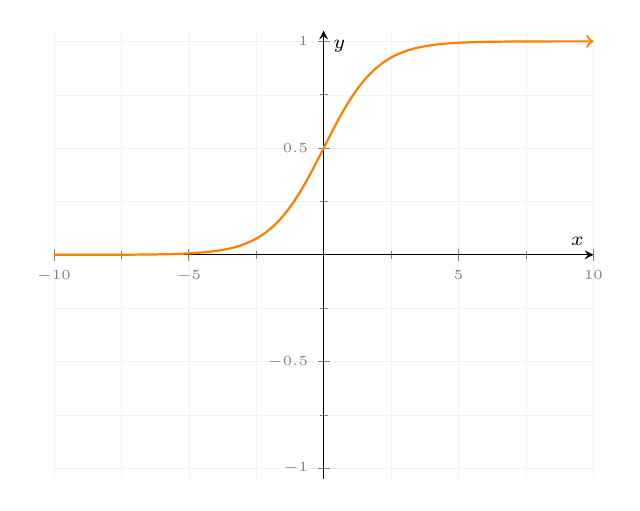
\begin{tikzpicture}
% axis settings {{{

\begin{axis}[
%	title          = graph_name,
	axis x line    = middle, % x-axis position
	axis y line    = middle, % y-axis position
	minor tick num = 1,      % num axis ticks
	grid           = both,
	grid style     =
	{
		line width=.1pt,
		draw=gray!10
	},
	xmax = 10,
	xmin = -10,
	ymax = 1.05, % 0.05 is to show the ->
	ymin = -1.05,
	tick label style = {
		font = \tiny,
		color = gray
	},
%	extra x ticks={3,1},
%	extra x tick labels={$\leftarrow$,$\rightarrow$},
%	extra y ticks={3,1},
%	extra y tick labels={$\leftarrow$,$\rightarrow$},
	legend style =
	{
		draw         = none, % remove legend bounding box
		font         = \tiny,
		legend pos   = outer north east,
		cells        = {anchor = west},
		fill         = gray,
		fill opacity = 0.4,
		text opacity = 1
	},
	xlabel       = {$\scriptstyle x$},
	ylabel       = {$\scriptstyle y$},
	xlabel style =
	{
		at     = {(ticklabel* cs:1)},
%		anchor = north west
	},
	ylabel style=
	{
		at     = {(ticklabel* cs:1)},
%		anchor = south west
	}
]
% }}}

\coordinate (O) at (0,0);

\addplot [
	domain=-10:10,
	no marks,
	samples=100,
	thick,
	orange,
	->
]
{1/(1+exp(-x)};
%\addlegendentry{$\frac{1}{1+e^{-x}}$};

\end{axis}
\end{tikzpicture}

% }}}

This is a function that will always output a value between 1 and 0 , i.e. , $ 0
\leq h_{\theta} (x) \leq 1 $. So we just take the output of our hypothesis
function , and pipe it through to the sigmoid in order to map it down to the
range we want. Which looks like :

\[
\begin{array}{ l@{} l@{} l@{} }
	h_\theta(x)
	& = g(\theta_0 + \theta_1 x) 
	& =
	\frac{1}
	{
		1+e^
		{
			-
			\left(
				\theta_0 + \theta_1 x
			\right)
		}
	}
	\\
	h_\theta(X)
	& = g(\Theta^T X)
	& =
	\frac{1}
	{
		1+e^
		{
			-
			\left(
				\Theta^T X
			\right)
		}
	}
	\\
\end{array}
\]

However $h_\theta(x) \in [0,1]$ or rather we are getting continuous values in
the interval between 0 and 1 and not really discrete values of 0 and 1 , which
is what the end goal of our binary classifier should be. Before we move on and
learn how to get discrete values , we should note that the values on this
continuous interval can also be considered useful. The hypothesis values on
this continuous interval represent the probability of x being in the positive
class. So the higher our $ h_\theta (x)$ value , the higher the probability
that x is 1 ( or true , or spam , or malignant etc ... )

\[
	\begin{array}{ l@{} l@{} }

	h_\theta(x) & = P(y=1|x;\theta)\\

	\end{array}
\]

\[
	\begin{array}{ l@{} l@{} }

	P(y=1|x;\theta) + P(y=0|x;\theta) & = 1 \\

	\end{array}
\]

These equations also show that now , our hypothesis $h_\theta$ is giving us a
probability value between 1 and 0 of how likely it is that our hypothesis is
true. The probability that the hypothesis is true is 0 at x = 0
and steadily increases as $x \rightarrow 1$. The function $h_\theta (x)$ is also
asymptotic at 1 and 0.

Anyway , what we actually want is an equation that classifies things into
groups of true or not true , and not an equation that predicts probabilities of
whether or not something is true. That is easy to do from what we already have.
All we have to do is come up with some \textbf{decision boundary} . This means
that if $x \geq \text{some threshold value}$ then we predict true or 1 , and if
$x > \text{some threshold value}$ then we predict false or 0. The equals can go
on either side of these two threshold values it doesn't really matter and is up
to you to set your own threshold values. One easy to pick threshold value is
just 0.5 (which is also the y intercept) , i.e., as long as $h_\theta (x) \geq
0.5 $ we will predict 1 (or true , or spam ...) and 0 otherwise.

\subsectionend
% }}} END SUB-SECTION : motivation
% 	SUB-SECTION : hypothesis_equation {{{
\subsection{Hypothesis Equation}
\label{ssec:hypothesis_equation}
\parindent=0em


\subsectionend
% }}} END SUB-SECTION : hypothesis_equation
% 	SUB-SECTION : cost_function {{{
\subsection{Cost Function}
\label{ssec:cost_function}
\parindent=0em

Training set :

\[
	\begin{array}{ l@{} l@{} }
	\left\{
		\left( x^{(1)},y^{(1)} \right),
		\left( x^{(2)},y^{(2)} \right),
		\left( x^{(3)},y^{(3)} \right),
		\ldots
		\left( x^{(m)},y^{(m)} \right)
	\right\}
	\end{array}
\]

where we have m samples / examples for each data point x :

\[
	\begin{array}{ l@{} l@{} }
	\begin{bmatrix}
		x_0 \\
		x_1 \\
		\vdots \\
		x_n \\
		\end{bmatrix}
		_{1 \times(n+1)}
	\in \mathbb{R}^{n+1}
	\; , \;
	x_0 = {1}
	\; , \;
	y \in {0,1}
	\end{array}
\]

There is no concept of residuals in logistic regression as compared to linear
regression. As a reminder a residual is the difference between the prdicted
value and the actual value. This doesnt make any sense as a concept when we are
trying to make discrete predictions.


This means that we cannot use least squares for figuring our how much error
there was in our prediction like we did in linear regression.


The new thing that we use is called Maximum Likelihood Estimation. The goal of
maximum likelihood is to find the optimal way to fit a distribution to the
data. Basically , whenever we have a data set we can fit a distribution to it.


So lets assume that the data you have can be fit according to a normal
distribution. But the quesiton is where and how do we center the normal
distribution. This is where maximum likelihood comes in. We basically just
start at 0 and go till our maximum value centering our distribution at each
value. The maximum likelihood equation tells us , how likely is it that this is
the correct center given the data that we have. We just do this for every value
possible in the range that we have for our values. Once we have tried (used the
likelihood function on) all of the locations possible for our center , we just
pick the center that gives the maximum output from the likelihood function.
Since in this example we are dealing with the normal distribution , 


~\footnote{ Good explainer video : 
\href{ https://www.youtube.com/watch?v=XepXtl9YKwc }{https://www.youtube.com/watch?v=XepXtl9YKwc }
}



Which means that we have a new cost function $J(\theta)$:


\[
	\begin{array}{ l@{} l@{} }
	J(\theta)
	& =
	\dfrac{1}{m}
	\sum_{i=1}^m
	\left\{
		\mathrm{Cost}(h_\theta(x^{(i)}),y^{(i)})
	\right\}
	\\
	\mathrm{Cost}(h_\theta(x),y)
	& =
	\left\{
		\begin{array}{ l@{} l@{} } 
			-\log(h_\theta(x))
			\;
			& \text{if y = 1} 
			\\ 
			-\log(1-h_\theta(x))
			\;
			& \text{if y = 0} 
		\end{array}
	\right.  
	\end{array}
\]

\[
	\begin{array}{ l@{} l@{} }
		\mathrm{Cost}(h_\theta(x),y)
		&
		\left\{
		\begin{array}{ l@{} l@{} l@{} }
			& = 0
			& \text{ if } h_\theta(x) = y
			\\
			& \rightarrow \infty
			&\text{ if } y = 0
			\; \mathrm{and} \;
			h_\theta(x) \rightarrow 1
			\\
			& \rightarrow \infty
			& \text{ if } y = 1
			\; \mathrm{and} \;
			h_\theta(x) \rightarrow 0
			\\
		\end{array}
	\right.
	\end{array}
\]


	Case y = 1

	
% ln(x)  {{{

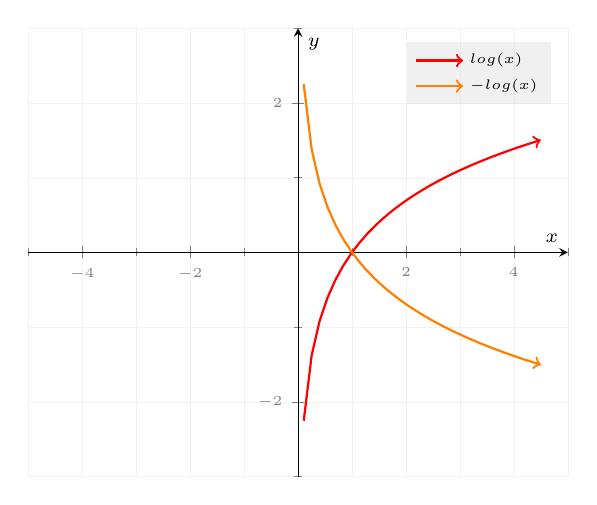
\begin{tikzpicture}
% axis settings {{{

\begin{axis}[
%	title          = graph_name,
	axis x line    = middle, % x-axis position
	axis y line    = middle, % y-axis position
	minor tick num = 1,      % num axis ticks
	grid           = both,
	grid style     =
	{
		line width = .1pt,
		draw       = gray!10
	},
	xmax      = 5,
	xmin      = -5,
	ymax      = 3,
	ymin      = -3,
	tick label style = {
		font  = \tiny,
		color = gray
	},
%	extra x ticks={3,1},
%	extra x tick labels={$\leftarrow$,$\rightarrow$},
%	extra y ticks={3,1},
%	extra y tick labels={$\leftarrow$,$\rightarrow$},
	legend style =
	{
		draw         = none, % remove legend bounding box
		font         = \tiny,
		legend pos   = north east,
		cells        = {anchor = west},
		fill         = gray!30,
		fill opacity = 0.4,
		text opacity = 1
	},
	xlabel       = {$\scriptstyle x$},
	ylabel       = {$\scriptstyle y$},
	xlabel style =
	{
		at     = {(ticklabel* cs:1)},
%		anchor = north west
	},
	ylabel style=
	{
		at     = {(ticklabel* cs:1)},
%		anchor = south west
	}
]
% }}}
\coordinate (O) at (0,0);

\addplot [
	domain=-10:4.5,
	samples=100,
	thick,
	red,
	->
]
{ln(x)};
\addlegendentry{$log(x)$};

\addplot [
	domain=-10:4.5,
	samples=100,
	thick,
	orange,
	->
]
{-ln(x)};
\addlegendentry{$-log(x)$};
\end{axis}
\end{tikzpicture}

% }}}
% ln(1-x)  {{{
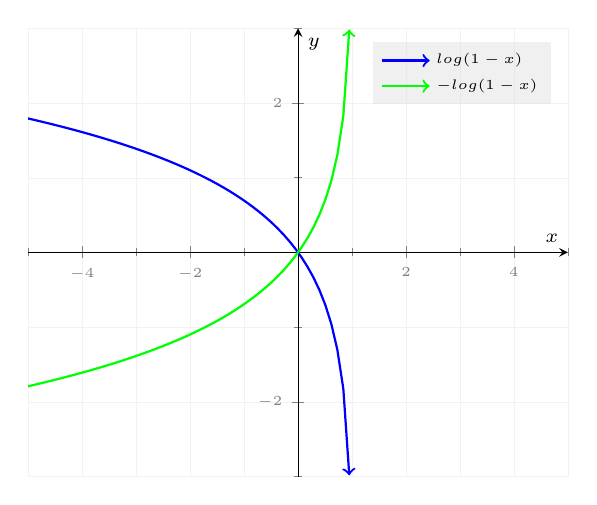
\begin{tikzpicture}
% axis settings {{{

\begin{axis}[
%	title          = graph_name,
	axis x line    = middle, % x-axis position
	axis y line    = middle, % y-axis position
	minor tick num = 1,      % num axis ticks
	grid           = both,
	grid style     =
	{
		line width = .1pt,
		draw       = gray!10
	},
	xmax      = 5,
	xmin      = -5,
	ymax      = 3,
	ymin      = -3,
	tick label style = {
		font  = \tiny,
		color = gray
	},
%	extra x ticks={3,1},
%	extra x tick labels={$\leftarrow$,$\rightarrow$},
%	extra y ticks={3,1},
%	extra y tick labels={$\leftarrow$,$\rightarrow$},
	legend style =
	{
		draw         = none, % remove legend bounding box
		font         = \tiny,
		legend pos   = north east,
		cells        = {anchor = west},
		fill         = gray!30,
		fill opacity = 0.4,
		text opacity = 1
	},
	xlabel       = {$\scriptstyle x$},
	ylabel       = {$\scriptstyle y$},
	xlabel style =
	{
		at     = {(ticklabel* cs:1)},
%		anchor = north west
	},
	ylabel style=
	{
		at     = {(ticklabel* cs:1)},
%		anchor = south west
	}
]
% }}}
\coordinate (O) at (0,0);

\addplot [
	domain=-10:0.95,
	samples=100,
	thick,
	blue,
	->
]
{ln(1-x)};
\addlegendentry{$log(1-x)$};

\addplot [
	domain=-10:0.95,
	samples=100,
	thick,
	green,
	->
]
{-ln(1-x)};
\addlegendentry{$-log(1-x)$};
\end{axis}
\end{tikzpicture}

% }}}
% ln(1-x)  {{{

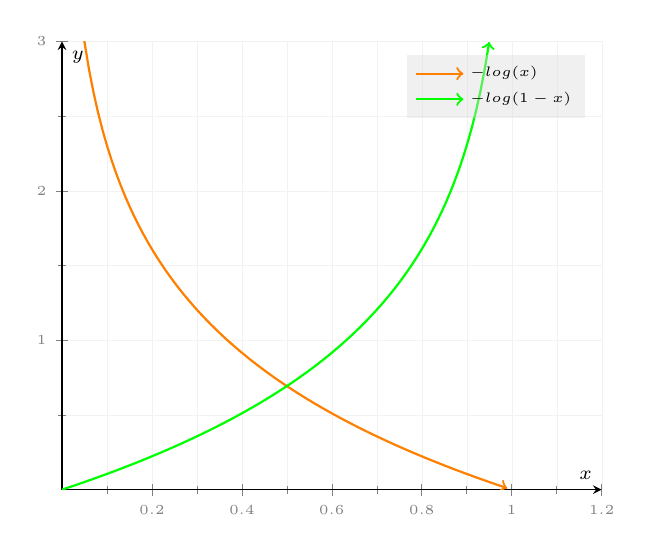
\begin{tikzpicture}
% axis settings {{{

\begin{axis}[
%	title          = graph_name,
	axis x line    = middle, % x-axis position
	axis y line    = middle, % y-axis position
	minor tick num = 1,      % num axis ticks
	grid           = both,
	grid style     =
	{
		line width = .1pt,
		draw       = gray!10
	},
	xmax      = 1.2,
	xmin      = 0,
	ymax      = 3,
	ymin      = 0,
	tick label style = {
		font  = \tiny,
		color = gray
	},
%	extra x ticks={3,1},
%	extra x tick labels={$\leftarrow$,$\rightarrow$},
%	extra y ticks={3,1},
%	extra y tick labels={$\leftarrow$,$\rightarrow$},
	legend style =
	{
		draw         = none, % remove legend bounding box
		font         = \tiny,
		legend pos   = north east,
		cells        = {anchor = west},
		fill         = gray!30,
		fill opacity = 0.4,
		text opacity = 1
	},
	xlabel       = {$\scriptstyle x$},
	ylabel       = {$\scriptstyle y$},
	xlabel style =
	{
		at     = {(ticklabel* cs:1)},
%		anchor = north west
	},
	ylabel style=
	{
		at     = {(ticklabel* cs:1)},
%		anchor = south west
	}
]
% }}}
\coordinate (O) at (0,0);

\addplot [
	domain=0:0.99,
	samples=100,
	thick,
	orange,
	->
]
{-ln(x)};
\addlegendentry{$-log(x)$};

\addplot [
	domain=0:0.95,
	samples=100,
	thick,
	green,
	->
]
{-ln(1-x)};
\addlegendentry{$-log(1-x)$};

\end{axis}
\end{tikzpicture}

% }}}

	Taking only the negative log from the graph and then using the interval
	only between $ 0 \leq x \leq 1$ , we get the following graph :

	Case y = 0
%	<img src="images/log_neg_interval.svg">
%	<img src="images/log_inv_neg_interval.svg">

\[
	\begin{array}{ l@{} l@{} l@{} } 
		\mathrm{Cost}(h_\theta(x),y)
		& = 0
		& \text{ if } h_\theta(x) = y 
		\\ 
		\mathrm{Cost}(h_\theta(x),y)
		& \rightarrow \infty
		&\text{ if } y = 0
		\; \mathrm{and} \;
		h_\theta(x) \rightarrow 1 
		\\ 
		\mathrm{Cost}(h_\theta(x),y)
		& \rightarrow \infty 
		& \text{ if } y = 1
		\; \mathrm{and} \;
		h_\theta(x) \rightarrow 0 
		\\ 
	\end{array}
\]

	\[
	\begin{array}{ l@{} l@{} } 
	J(\theta)
	& =
	\dfrac{1}{m}
	\sum_{i=1}^m
	\left\{
		\mathrm{Cost}(h_\theta(x^{(i)}),y^{(i)})
	\right\} 
	\\ 
	\mathrm{Cost}(h_\theta(x),y)
	& =
	\left\{ 
		\begin{array}{ l@{} l@{} } 
			-\log(h_\theta(x))
			\;
			& \text{if y = 1} 
			\\ 
			-\log(1-h_\theta(x))
			\;
			& \text{if y = 0} 
		\end{array}
	\right.  
	\\ 
	& = 
	-y\log(h_\theta(x))
	+
	(1-y)\log(1-h_\theta(x)) 
	\end{array}
\]


\[
	\begin{array}{ l@{} l@{} } 
	J(\theta)
	& =
	{ \displaystyle 
		\dfrac{1}{m}
		\sum_{i=1}^m
		\left\{
			\mathrm{Cost}(h_\theta(x^{(i)}),y^{(i)})
		\right\}
	}
	\\ 
	& =
	\dfrac{1}{m} 
	{ \displaystyle 
		\left(
			\sum_{i=1}^m
			\left\{
				-y^{(i)}\log(h_\theta(x^{(i)}))
				+
				(1-y^{(i)})\log(1-h_\theta(x^{(i)}))
			\right\}
		\right)
	} 
	\end{array}
\]

\subsectionend
% }}} END SUB-SECTION : cost_function
% 	SUB-SECTION : gradient_descent {{{
\subsection{Gradient Descent}
\label{ssec:gradient_descent}
\parindent=0em

	<h3>Logistic Regression : Gradient Descent</h3>

Just for reference cause we will need it later.

\[
	\begin{array}{ l@{} l@{} }
		\nabla J(\Theta)
		& =
		\left\langle
		  {\displaystyle \frac{\partial}{\partial \theta_0} J(\Theta)}
		, {\displaystyle \frac{\partial}{\partial \theta_1} J(\Theta)}
		, {\displaystyle \frac{\partial}{\partial \theta_2} J(\Theta)}
		\ldots
		, {\displaystyle \frac{\partial}{\partial \theta_m} J(\Theta)}
		\right\rangle
		\\
	\end{array}
\]


\[
	\begin{array}{ l@{} l@{} }
\sigma(x)             & = \frac{1}{1+e^{-x}} \\
\frac{d}{dx}\sigma(x) & = \frac{d}{dx} \left(  \frac{1}{1+e^{-x} } \right) \\
                      & = \frac{0 \cdot(1+e^{-x}) - (-e^{-x}) \cdot 1}{ ( 1+e^{-x} ) ^2} \text{$\hspace{46 mm}$Quotient rule}\\
                      & = \frac{e^{-x}}{ ( 1+e^{-x} ) ^2}  \\
                      & = \frac{(1+e^{-x}) -1 }{ ( 1+e^{-x} ) ^2} \\
                      & = \frac{ (1+e^{-x})}{ ( 1+e^{-x} ) ^2}  - \left( \frac{1}{1+e^{-x}} \right)^2\\
                      & = \frac{1}{1+e^{-x}}  - \left( \frac{1}{1+e^{-x}} \right)^2\\
                      & = \sigma (x) - \sigma(x)^2\\
\sigma^{'} (x)        & = \sigma(x)(1-\sigma(x))
	\end{array}
\]


We also have the following :
\[
	\begin{array}{ l@{} l@{} } 
		h_\theta(\Theta^T x)
		= \sigma(\Theta^Tx)
		& = \frac{1}{1+e^{-\Theta^T x}} \\ 
	\end{array}
\]

\[
\begin{array}{ l@{} l@{} l@{} l@{} } 
		P(y^{(i)} = 1 | x^{(i)} ; \theta)
		& = h_\theta(x)
		& = \sigma(x)
		& = \frac{1}{1+e^{-x}}
		\\ 
		P(y^{(i)} = 0 | x^{(i)} ; \theta)
		& = 1 - h_\theta(x)
		& = 1 - \sigma(x)
		& = 1 - \frac{1}{1+e^{-x}}
		\\ 
	\end{array}
\]

This gives us the overall likelihood of any outcome y given x and theta as :

\[
\begin{array}{ l@{} l@{} l@{} } 
		L(\theta) 
		& = P(y^{(i)}| x^{(i)} ; \theta)
		& = h(x^{(i)})^{y^{(i)}} \cdot ( 1 - h(x^{(i)}))^{1 - y^{(i)}} 
	\end{array}
\]

overall i's

\[
	\begin{array}{ l@{} l@{} }
	L(\theta) & =
	{ \displaystyle \prod_{i=1}^{m} }
	\left\{
		h
		\left(x^{(i)}\right)
		^{
			\left(
				y^{(i)}
			\right)
		}
		\cdot
		\left(
			1 - h(x^{(i)})
		\right)
		^{
			\left(
				1 - y^{(i)}
			\right)
		}
	\right\}
	\\
	\log(L(\theta)) & = \mathscr{L}(\theta) \\ 
	\mathscr{L}(\theta)
	& =
	\log \left( 
	{ \displaystyle \prod_{i=1}^{m} }
	\left\{
		h
		\left(x^{(i)}\right)
		^{
			\left(
				y^{(i)}
			\right)
		} 
		\cdot 
		\left(
			1 - h(x^{(i)})
		\right)
		^{
			\left(
				1 - y^{(i)}
			\right)
		} 
	\right\} 
	\right) 
	\\ 
	& = 
	{ \displaystyle \sum_{i=1}^{m} } \left\{ 
		\log \left( 
			h
			\left(x^{(i)}\right)
			^{
				\left(
					y^{(i)}
				\right)
			} 
			\cdot 
			\left(
				1 - h(x^{(i)})
			\right)
			^{
				\left(
					1 - y^{(i)}
				\right)
			} 
		\right) 
	\right\} 
	\\ 
	& = 
	{ \displaystyle \sum_{i=1}^{m} } \left\{ 
		\log \left( 
			h
			\left(x^{(i)}\right)
			^{
				\left(
					y^{(i)}
				\right)
			} 
		\right) 
		+ 
		\log \left( 
			\left(
				1 - h(x^{(i)})
			\right)
			^{
				\left(
					1 - y^{(i)}
				\right)
			} 
		\right) 
	\right\} 
	\\ 
	& = 
	{ \displaystyle \sum_{i=1}^{m} } \left\{ 
		\left(
			y^{(i)}
		\right) 
		\cdot 
		\log \left( 
		h \left(
			x^{(i)}
		\right) 
		\right) 
		+ 
		\left(
			1 - y^{(i)}
		\right) 
		\cdot 
		\log \left( 
		\left(
			1 -
			h \left(
				x^{(i)}
			\right) 
		\right) 
		\right) 
	\right\} 
	\end{array}
\]

We want to maximize the likelihood so we take the derivative :


\[
	\begin{array}{ l@{} l@{} r@{} } 
	{ \displaystyle \frac{\partial}{\partial \theta}}
	\mathscr{L}(\theta) 
	& = 
	{ \displaystyle \frac{\partial}{\partial \theta}}
	\left(
		{ \displaystyle \sum_{i=1}^{m} } \left\{ 
			\left(
				y^{(i)}
			\right) 
			\cdot 
			\log \left( 
			h \left(
				x^{(i)}
			\right) 
			\right) 
			+ 
			\left(
				1 - y^{(i)}
			\right) 
			\cdot 
			\log \left( 
			\left(
				1 -
				h \left(
					x^{(i)}
				\right) 
			\right) 
			\right) 
		\right\}
	\right) 
	\\ 
	& = 
	{ \displaystyle \frac{\partial}{\partial \theta}}
	\left(
		{ \displaystyle \sum_{i=1}^{m} } \left\{ 
			\left(
				y^{(i)}
			\right) 
			\cdot 
			\log \left( 
			\sigma \left(
				x^{(i)}
			\right) 
			\right) 
			+ 
			\left(
				1 - y^{(i)}
			\right) 
			\cdot 
			\log \left( 
			\left(
				1 -
				\sigma \left(
					x^{(i)}
				\right) 
			\right) 
			\right) 
		\right\}
	\right) 
	\\ 
	& = 
	{ \displaystyle \sum_{i=1}^{m} } \left\{ 
		\left(
			y^{(i)}
		\right) 
		\cdot 
		{ \displaystyle \frac{\partial}{\partial \theta}} \left( 
			\log \left( 
			\sigma \left(
				x^{(i)}
			\right) 
			\right) 
		\right) 
		+ 
		\left(
			1 - y^{(i)}
		\right) 
		\cdot 
		{ \displaystyle \frac{\partial}{\partial \theta}} \left( 
			\log \left( 
			\left(
				1 -
				\sigma \left(
					x^{(i)}
				\right) 
			\right) 
		\right) 
	\right\} 
	\right) 
	\\ 
	& = 
	{ \displaystyle \sum_{i=1}^{m} } \left\{ 
		\left(
			y^{(i)}
		\right) 
		\cdot 
		\left( 
			{ \displaystyle
			\frac
				{
					1
				}
				{
					\sigma \left( x^{(i)} \right)
				}
			} 
			\cdot 
			\sigma \prime \left( x^{(i)} \right) 
		\right) 
		+ 
		\left( 1 - y^{(i)} \right) 
		\cdot 
		\left( 
			{ \displaystyle
			\frac
				{
					1
				}
				{
					1 - \sigma \left( x^{(i)} \right)
				}
			} 
			\cdot 
			- \sigma \prime \left( x^{(i)} \right) 
		\right) 
	\right\} 
	& \text{Chain Rule} 
	\\ 
	& = 
	\end{array}
\]

Gradient Descent

\[
	\begin{array}{ l@{} l@{} } 
		\frac{\partial}{\partial \theta_0} J(\Theta)
		& =
		\left(
			\frac{1}{m}
			\cdot
			\sum_{i=1}^m \left\{
					\left(
						h_\theta(x^{(i)}) - y^{(i)}
					\right)^{2}
					\cdot
					x_{0}^{(i)}
			\right\}
		\right) 
		\\ 
		\frac{\partial}{\partial \theta_j} J(\Theta)
		& =
		\left(
			\frac{1}{m} \cdot
			\sum_{i=1}^m \left\{
				\left(
					h_\theta(x^{(i)}) - y^{(i)}
				\right)^{2}
				\cdot
				x_{j}^{(i)}
			\right\}
		\right) 
		+ 
		\frac{\lambda}{m}\cdot \theta_j 
		\\ 
	\end{array}
\]

The second sum, 
\( \frac{\lambda}{2m}
   \sum_{j = 1}^{n} {\theta_{j}^{2}} \)
means to explicitly exclude the bias term, $\theta_0$. i.e. the $\theta$
vector is indexed from 0 to n (holding n+1 values, $\theta_0$ through
$\theta_n$), and this sum explicitly skips $\theta_0$, by
running from 1 to n, skipping 0. Thus, when computing the equation, we should
continuously update the two following equations:

	\[
	\begin{array}{ l@{} l@{} l@{} l@{} } 
		\theta_0
		& := &
		\theta_0
		- \alpha
		\cdot
		\left(
		\frac{1}{m}
		\cdot 
			\sum_{i=1}^m
			\left\{
				\left(
					h_\theta(x^{(i)}) - y^{(i)}
				\right)^{2}
				\cdot
				x_{0}^{(i)}
			\right\}
		\right) 
		\hspace{0.5cm} & \text{for} \; j = 0 
		\\ 
		\theta_j
		& := &
		\theta_j
		- \alpha
		\cdot
		\left(
		\frac{1}{m}
		\cdot 
			\sum_{i=1}^m
			\left\{
				\left(
					h_\theta(x^{(i)}) - y^{(i)}
				\right)^{2}
				\cdot
				x_{j}^{(i)}
				+
				\left(
					\frac{\lambda}{m}\cdot \theta_j
				\right)
			\right\}
		\right) 
		\hspace{0.5cm} & \text{for} \; j = 1,2, \ldots , n 
		\\ 
		& :=
		& \theta_j
		\cdot
		(1 - \alpha \cdot \frac{\lambda}{m})
		-
		\alpha
		\cdot
		\left(
		\frac{1}{m}
		\cdot 
			\sum_{i=1}^m
			\left\{
				\left(
					h_\theta(x^{(i)}) - y^{(i)}
				\right)^{2}
				\cdot
				x_{j}^{(i)} 
			\right\}
		\right) 
		\\ 
		\end{array}
	\]
\subsectionend
% }}} END SUB-SECTION : gradient_descent
% 	SUB-SECTION : extra {{{
\subsection{Extra}
\label{ssec:extra}
\parindent=0em

% 		SUB-SUB-SECTION : advanced_optimization_algorithms {{{
\subsubsection{Advanced Optimization Algorithms}
\label{sssec:advanced_optimization_algorithms}
\parindent=0em


	<h3>Advanced Optimization Algorithms</h3>

	The various advanced optimization algorithms are :


	<ul>
		<li>Gradient Descent</li>
		<li>Conjugate gradient</li>
		<li>BFGS</li>
		<li>L-BFGS</li>
	</ul>

\subsubsectionend
% }}} END SUB-SUB-SECTION : advanced_optimization_algorithms
% 		SUB-SUB-SECTION : multiclass_classification {{{
\subsubsection{Multiclass Classification}
\label{sssec:multiclass_classification}
\parindent=0em

	<h3>Logistic Regression : Multiclass Classification</h3>

	<p>

		To do multiclass classification , we use a method called one-vs-all (
		sometimes also called one-vs-rest ). In this method we will train a new
		classfier with a spereate hypothesis function $h_\theta(x)$ for each
		thing we want to classify.  So if we want to classify k different things
		, we will have k different hypothesis functions. These will be denoted
		using a superscript $h_\theta^{(k)}(x)$.
		
		
		\[
			\begin{array}{ l@{} l@{} }
				h_\theta^{(i)}(x) = P(y=i|x;\theta) \; , \; 1 \leq i \leq k , k
				\in \mathbb{N}
			\end{array}
		\]


		The probability equation is telling us what the probability is that the
		x value we are looking at belongs in the current class k. <br> <br>

		What this means is that for each class k , when we recieve a new data
		point we dont have to decide which specific class it belongs into yet.
		All we have to do is figure out if it belongs in the current class that
		we are looking at. So does it belong in the current class or one of all
		of the rest of the classes , doesnt matter which. Then we repeat this
		process until we figure out which one it belongs to , by iterative
		comparison of one-vs-all.  <br> <br>

		So at the end we just pick the hypothesis that maximizes the probability
		that a given item x belongs in class k : 
		
		\[
			\begin{array}{ l@{} l@{} }
				\max\limits_i h_\theta^{(i)}(x) &
			\end{array}
		\]

	</p>


\subsubsectionend
% }}} END SUB-SUB-SECTION : multiclass_classification
% 		SUB-SUB-SECTION : overfitting {{{
\subsubsection{Overfitting}
\label{sssec:overfitting}
\parindent=0em

	<h3>Overfitting</h3>

	If we have too many features , the learned hypothesis may fit the training
	set very well , i.e. , 

	\[
		\begin{array}{ l@{} l@{} }


			J(\theta)
			= \frac{1}{2m}
			\sum_{i=1}^m
			\left\{
				\left(
					h_\theta(x^{(i)}) - y^{(i)}
				\right)^{2}
			\right\}

			\approx 0


		\end{array}
	\]

	but this function may fail to generalize to new examples.<br> <br>

	<b> Underfitting </b>, or <b> high bias </b>, is when the form of our
	hypothesis function h maps poorly to the trend of the data. It is usually
	caused by a function that is too simple or uses too few features.<br> <br>

	At the other extreme, <b> overfitting </b>, or <b> high variance </b>, is
	caused by a hypothesis function that fits the available data but does not
	generalize well to predict new data. It is usually caused by a complicated
	function that creates a lot of unnecessary curves and angles unrelated to
	the data.<br> <br>

	There are a couple of things we can do to reduce over fitting :


	<ol>
		<li>Reduce number of features</li>
		<ol>
			<li>Manually select which features to keep</li>
			<li>Use a model selection algorithm</li>
		</ol>
		<li>Use Regularization</li>
		<ol>
			<li>Keep all the features , but reduce the magnitude / values of the
				parameters $\theta_j$ </li>
			<li>Works well when we have a lot of features , each one of whic
				contribute a little bit towards predictin $y$</li>
		</ol>
	</ol>


\subsubsectionend
% }}} END SUB-SUB-SECTION : overfitting
% 		SUB-SUB-SECTION : regularization {{{
\subsubsection{Regularization}
\label{sssec:regularization}
\parindent=0em

<h3>Regularization</h3>

To fix the problem of overfitting one of the things that we prefer is for the
hypothesis to be as simple as possible. This means that we want to reduce the
effect ( as close to zero as we can ) of the higher order polynomials as we can.
In order to do this we can introduce a regularization term. The purpose of this
term is to penalize the cost function (by assigning a higher value) when it
assigns higher weight ( larger values for $\theta_j$ ) to higher order
polynomials. This means the higher the order of the $x$ value the more the cost
function will be rewarded if it DOES NOT include it as a significant contibutor.
Keep in mind we are using the same amount of features $x_(j)^{(i)}$ , all we are
doing is reducing the polynomial order of the features. The cost function is not
being penalized for reducing the impact of the features theselves.<br>

The regularization term looks like :

\[
	\begin{array}{ l@{} l@{} } 
		\frac{1}{2} \cdot
		\frac{1}{m} \cdot 
		\lambda \cdot
		\sum_{j = 1}^{n}
		\left\{
			{\theta_{j}^{2}}
		\right\} 
	\end{array}
\]

$\lambda$ is called the regularization parameter. Its job is to control the
tradeoff between two different goals. The first goal is to actually fit the
training data well. This is done by our original cost function $J(\theta)$. The
second goal is to keep the parameters small. This makes our Cost function now
look like :

\[
	\begin{array}{ l@{} l@{} } 
		J(\theta)
		=
		\left( 
		\frac{1}{2}
		\cdot
		\frac{1}{m}
		\cdot 
			\left(
				\sum_{i=1}^m
				\left\{
					\left(
						h_\theta(x^{(i)}) - y^{(i)}
					\right)^{2}
				\right\}
			\right) 
			+
			\left( 
				\frac{1}{2} \cdot
				\frac{1}{m} \cdot 
				\lambda \cdot
				\sum_{j = 1}^{n}
				\left\{
					{\theta_{j}^{2}}
				\right\}
			\right)
		\right) 
	\end{array} 
\]


Keep in mind though that if we set \( lambda \) to be some huge value like


\( \lambda = 10^{10} \) then we might not even achieve our primary objective of
fitting the data well since we are punishing the cost function too much. This
would basically mean that each \( \theta_j \approx 0 \; , \; j \geq 1 \) and we
would effectively only be left with \( h_{\theta}(x) = \theta_0 \) which is
basically just a straight line through the intercept.  This would result in a
case of underfitting due to a too large \( \lambda \) value.

	<h3>Regularized Linear Regression</h3>

	\[
		\begin{array}{ l@{} l@{} } 
			\min\limits_\theta
			J(\theta)
			=
			\frac{1}{2}
			\cdot
			\frac{1}{m}
			\cdot
			\left(
				\left(
					\sum_{i=1}^m
					\left\{
						\left(
							h_\theta(x^{(i)}) - y^{(i)}
						\right)^{2}
					\right\}
				\right) 
				+
				\left( 
					\frac{1}{2} \cdot
					\frac{1}{m} \cdot
					\lambda \cdot
					\sum_{j = 1}^{n}
					\left\{
						{\theta_{j}^{2}}
					\right\}
				\right)
			\right) 
		\end{array} 
	\]


\subsubsectionend
% }}} END SUB-SUB-SECTION : regularization

\subsectionend
% }}} END SUB-SECTION : extra

%	{{{
<h3>Logistic Regression</h3>

This is a type of classification algorithm , as opposed to linear or non-linear
regression algorithms which all relied on predicting continuous values , a
classifcation algirthm will use the independent variables (features) to predict
binary values like : Yes / No , True / False , Malignant / Non-Malignant ,
Pregnant / Not-Pregnant etc... All these examples are binary beacuse that is
what I am going to be using in this explanation , but we can use multiple
logistic regression with vectors to extend the algorithm for multi-class
classification to classify the output into as many fields as we like.<br>

Even though the dependant variables are discrete classifications , the
independant variables $x_j$ values should all be continous.<br>

Logistic Regression measures the probability of a case belonging to a specific
class. Logistic Regression can be used to understand the impact of a feature on
a dependant variable. <br>

<ul>

	<li>Input / independant Variables : $ X \in \mathbb{R}^{m \times n}$</li>
	<li>Output / dependant Variables : $ y \in \{0,1\}$</li>
	<li>: $ \hat{y} = P(y=1|x) $</li>
	<li>: $ P(y=0|x) = 1 - P(y=1|x) $</li>
</ul>

We can use the equations we have from linear regression as outr starting poing
for logistic regression. We have :

			\[
				\begin{array}{ l@{} l@{}} 
				\Theta_{(n \times 1)} = 
				\begin{bmatrix} 
				\theta_0 \\
				\theta_1 \\
				\theta_2 \\
				\vdots \\
				\theta_n \\ 
				\end{bmatrix} 
				\; , \; 
				\Theta_{(1 \times n)}^{T} = 
				\begin{bmatrix} 
				\theta_0 ,
				\theta_1 ,
				\theta_2 ,
				\cdots , 
				\theta_n
				\end{bmatrix} 
				\; , \; 
				X_{(n \times 1)} = 
				\begin{bmatrix} 
					1 \\
					x_1 \\
					x_2 \\
					\vdots \\
					x_n \\ 
				\end{bmatrix} \\ 
				\end{array}
			\]

			\[
			\begin{array}{ l@{} l@{} l@{} l@{} } 
			\hat{y}
			& = h_\theta (x)
			& = \Theta_{(1 \times n)}^{T} \cdot X_{(n \times 1)} 
			& = 
			\begin{bmatrix} 
				\theta_0 \\
				\theta_1 \\
				\theta_2 \\
				\vdots \\
				\theta_n \\ 
			\end{bmatrix}_{(1 \times n)} 
			\cdot 
			\begin{bmatrix} 
				1 \\
				x_1 \\
				x_2 \\
				\vdots \\
				x_n \\ 
			\end{bmatrix}_{(n \times 1)} 
			\\ 
			& & & =
			\begin{bmatrix} 
				x_0\theta_0 +
				x_1\theta_1 +
				x_2\theta_2 +
				\cdots +
				x_n\theta_n \\ 
			\end{bmatrix}_{(1 \times 1)} 
			\end{array}
			\] 

\[
	\begin{array}{ l@{} l@{} l@{}} 
		\Theta^T X & = & \theta_0 x_0 + \theta_1 x_1 + \theta_2 x_2 + \ldots +
		\theta_n x_n \\
		h_\theta (x) & = & \Theta^T X \\ 
	\end{array}
\]

<h4>The Training Process</h4>

<ol>
	<li>Initialize $\theta$</li>
	<li>Calculate $ \hat{y} = \sigma(\Theta^{T} X)$</li>
	<li>Compare the output of $\hat{y}$ with actual output of cutomer , y, and
		record it as error.</li>
	\[
		\begin{array}{ l@{} l@{} } 
			Error = 1 - 
			\left(
				\hat{y} = \sigma(\theta^{T} X)
			\right)
		\end{array}
	\]
	<li>Calcualte error for all customers $Cost = J(\theta)$</li>
	<li>Change $\theta$ to reduce the cost</li>
	<li>Go back to step 2</li>
</ol>

\[
	\begin{array}{ l@{} l@{} } 
	\widehat{y} = \sigma(\theta_1 x_1 + \ldots + \theta_n x_n) 
	\end{array}
\]

\[
	\begin{array}{ l@{} l@{} } 
		J(\theta)
		& =
		-
		\frac{1}{m}
		\cdot
		\sum_{i=1}^{m}
		\left\{
			y^{i}
			log(\widehat{y^{i}})
			+
			(1 - y^{i})
			log(1-\widehat{y^{i}})
		\right\}
	\end{array}
\]

\[
	\begin{array}{ l@{} l@{} } 
		\frac{\partial}{\partial \theta_0} J(\theta_1)
		& =
		-
		\frac{1}{m}
		\cdot 
		\sum_{i=1}^m
		\left\{
			\left(
				y^{i} - \widehat{y^{i}}
			\right)
			\cdot
			x_{1}^{i}
		\right\} 
	\end{array}
\]

Using gradient descent the gradient vector is :

\[
	\begin{array}{ l@{} l@{} } 
		\nabla J
		& = 
		\begin{bmatrix} 
			\frac{\partial J(\theta_1)}{\partial \theta_1}  \\ 
			\frac{\partial J(\theta_2)}{\partial \theta_2}  \\ 
			\vdots \\ 
			\frac{\partial J(\theta_k)}{\partial \theta_k}  \\ 
		\end{bmatrix} 
	\end{array}
\]

update equation :

\[
	\begin{array}{ l@{} l@{} } 
	\theta_{new} = \theta_{prev} - \eta \nabla J 
	\end{array}
\]


%	  }}}


%\sectionend
% }}} END SECTION : logistic_regression




% ----------------------------------------------------------------------------- 
\bibliography{1_bibliography/references}
\end{document}
% =============================================================================
% - EOF - EOF - EOF - EOF - EOF - EOF - EOF - EOF - EOF - EOF - EOF - EOF -
% =============================================================================

